\documentclass{article}\usepackage[]{graphicx}\usepackage[]{color}
% maxwidth is the original width if it is less than linewidth
% otherwise use linewidth (to make sure the graphics do not exceed the margin)
\makeatletter
\def\maxwidth{ %
  \ifdim\Gin@nat@width>\linewidth
    \linewidth
  \else
    \Gin@nat@width
  \fi
}
\makeatother

\definecolor{fgcolor}{rgb}{0.345, 0.345, 0.345}
\newcommand{\hlnum}[1]{\textcolor[rgb]{0.686,0.059,0.569}{#1}}%
\newcommand{\hlstr}[1]{\textcolor[rgb]{0.192,0.494,0.8}{#1}}%
\newcommand{\hlcom}[1]{\textcolor[rgb]{0.678,0.584,0.686}{\textit{#1}}}%
\newcommand{\hlopt}[1]{\textcolor[rgb]{0,0,0}{#1}}%
\newcommand{\hlstd}[1]{\textcolor[rgb]{0.345,0.345,0.345}{#1}}%
\newcommand{\hlkwa}[1]{\textcolor[rgb]{0.161,0.373,0.58}{\textbf{#1}}}%
\newcommand{\hlkwb}[1]{\textcolor[rgb]{0.69,0.353,0.396}{#1}}%
\newcommand{\hlkwc}[1]{\textcolor[rgb]{0.333,0.667,0.333}{#1}}%
\newcommand{\hlkwd}[1]{\textcolor[rgb]{0.737,0.353,0.396}{\textbf{#1}}}%
\let\hlipl\hlkwb

\usepackage{framed}
\makeatletter
\newenvironment{kframe}{%
 \def\at@end@of@kframe{}%
 \ifinner\ifhmode%
  \def\at@end@of@kframe{\end{minipage}}%
  \begin{minipage}{\columnwidth}%
 \fi\fi%
 \def\FrameCommand##1{\hskip\@totalleftmargin \hskip-\fboxsep
 \colorbox{shadecolor}{##1}\hskip-\fboxsep
     % There is no \\@totalrightmargin, so:
     \hskip-\linewidth \hskip-\@totalleftmargin \hskip\columnwidth}%
 \MakeFramed {\advance\hsize-\width
   \@totalleftmargin\z@ \linewidth\hsize
   \@setminipage}}%
 {\par\unskip\endMakeFramed%
 \at@end@of@kframe}
\makeatother

\definecolor{shadecolor}{rgb}{.97, .97, .97}
\definecolor{messagecolor}{rgb}{0, 0, 0}
\definecolor{warningcolor}{rgb}{1, 0, 1}
\definecolor{errorcolor}{rgb}{1, 0, 0}
\newenvironment{knitrout}{}{} % an empty environment to be redefined in TeX

\usepackage{alltt}
\usepackage[top=1in,bottom=1in,left=1in,right=1in]{geometry}

\usepackage{setspace}

\usepackage{hyperref}
\hypersetup{colorlinks=true, urlcolor=blue, breaklinks=true}

\newcommand{\link}[1]{\footnote{\color{blue}\href{#1}{#1}}}
\newcommand{\myhref}[1]{\href{#1}{#1}}

\usepackage{amsmath}
\usepackage{amssymb}
\usepackage{mathtools}
\usepackage{linguex}
\usepackage{natbib}

%\usepackage{Sweave}





% The package for linguistics examples

\title{Plot and examine chains: 3 regions (FP + reg)}
\author{JD}
\IfFileExists{upquote.sty}{\usepackage{upquote}}{}
\begin{document}
\maketitle

\section{Simple model and plots}

This file collects draws and generates plots and info about parameters.

\begin{knitrout}
\definecolor{shadecolor}{rgb}{0.969, 0.969, 0.969}\color{fgcolor}\begin{kframe}
\begin{alltt}
\hlstd{burnin} \hlkwb{<-} \hlnum{200}

\hlkwd{library}\hlstd{(dplyr)}
\end{alltt}


{\ttfamily\noindent\itshape\color{messagecolor}{\#\# \\\#\# Attaching package: 'dplyr'}}

{\ttfamily\noindent\itshape\color{messagecolor}{\#\# The following objects are masked from 'package:stats':\\\#\# \\\#\#\ \ \ \  filter, lag}}

{\ttfamily\noindent\itshape\color{messagecolor}{\#\# The following objects are masked from 'package:base':\\\#\# \\\#\#\ \ \ \  intersect, setdiff, setequal, union}}\begin{alltt}
\hlkwd{library}\hlstd{(rstan)}
\end{alltt}


{\ttfamily\noindent\itshape\color{messagecolor}{\#\# Loading required package: StanHeaders}}

{\ttfamily\noindent\itshape\color{messagecolor}{\#\# Loading required package: ggplot2}}

{\ttfamily\noindent\itshape\color{messagecolor}{\#\# Need help getting started? Try the R Graphics Cookbok:\\\#\# https://r-graphics.org}}

{\ttfamily\noindent\itshape\color{messagecolor}{\#\# rstan (Version 2.21.1, GitRev: 2e1f913d3ca3)}}

{\ttfamily\noindent\itshape\color{messagecolor}{\#\# For execution on a local, multicore CPU with excess RAM we recommend calling\\\#\# options(mc.cores = parallel::detectCores()).\\\#\# To avoid recompilation of unchanged Stan programs, we recommend calling\\\#\# rstan\_options(auto\_write = TRUE)}}\begin{alltt}
\hlstd{c1} \hlkwb{<-} \hlkwd{read.csv}\hlstd{(}\hlstr{"chain1/chain-0.csv"}\hlstd{)}

\hlstd{dataf} \hlkwb{<-} \hlkwd{select}\hlstd{(c1,} \hlkwd{starts_with}\hlstd{(}\hlstr{"mu_rt"}\hlstd{))}

\hlstd{dataf} \hlkwb{<-} \hlstd{dataf[burnin}\hlopt{:}\hlkwd{length}\hlstd{(dataf[,} \hlnum{1}\hlstd{]), ]}

\hlkwd{str}\hlstd{(dataf)}
\end{alltt}
\begin{verbatim}
## 'data.frame':	2794 obs. of  12 variables:
##  $ mu_rt__0 : num  259 259 249 251 251 ...
##  $ mu_rt__1 : num  320 320 302 314 314 ...
##  $ mu_rt__2 : num  745 744 705 718 716 ...
##  $ mu_rt__3 : num  259 259 249 251 251 ...
##  $ mu_rt__4 : num  339 339 316 338 338 ...
##  $ mu_rt__5 : num  753 752 713 723 721 ...
##  $ mu_rt__6 : num  265 264 252 255 255 ...
##  $ mu_rt__7 : num  322 322 304 315 315 ...
##  $ mu_rt__8 : num  768 775 735 746 744 ...
##  $ mu_rt__9 : num  265 264 252 255 255 ...
##  $ mu_rt__10: num  341 341 318 339 339 ...
##  $ mu_rt__11: num  766 770 730 740 739 ...
\end{verbatim}
\begin{alltt}
\hlstd{dataf2} \hlkwb{<-} \hlkwd{select}\hlstd{(c1,} \hlkwd{starts_with}\hlstd{(}\hlstr{"mu_reg"}\hlstd{))}

\hlstd{dataf2} \hlkwb{<-} \hlstd{dataf2[burnin}\hlopt{:}\hlkwd{length}\hlstd{(dataf2[,} \hlnum{1}\hlstd{]), ]}

\hlkwd{str}\hlstd{(dataf2)}
\end{alltt}
\begin{verbatim}
## 'data.frame':	2794 obs. of  12 variables:
##  $ mu_reg__0 : num  0.0318 0.0318 0.0318 0.0341 0.0341 ...
##  $ mu_reg__1 : num  0.0502 0.0502 0.0502 0.0516 0.0516 ...
##  $ mu_reg__2 : num  0.481 0.481 0.481 0.485 0.485 ...
##  $ mu_reg__3 : num  0.0187 0.0187 0.0187 0.0201 0.0201 ...
##  $ mu_reg__4 : num  0.0504 0.0504 0.0504 0.0518 0.0518 ...
##  $ mu_reg__5 : num  0.467 0.468 0.468 0.476 0.476 ...
##  $ mu_reg__6 : num  0.255 0.156 0.156 0.16 0.16 ...
##  $ mu_reg__7 : num  0.242 0.242 0.242 0.247 0.247 ...
##  $ mu_reg__8 : num  0.474 0.469 0.469 0.476 0.476 ...
##  $ mu_reg__9 : num  0.306 0.206 0.206 0.211 0.211 ...
##  $ mu_reg__10: num  0.273 0.273 0.273 0.278 0.278 ...
##  $ mu_reg__11: num  0.503 0.507 0.507 0.516 0.516 ...
\end{verbatim}
\begin{alltt}
\hlstd{c2} \hlkwb{<-} \hlkwd{read.csv}\hlstd{(}\hlstr{"chain2/chain-0.csv"}\hlstd{)}

\hlstd{dataf.c2} \hlkwb{<-} \hlkwd{select}\hlstd{(c2,} \hlkwd{starts_with}\hlstd{(}\hlstr{"mu_rt"}\hlstd{))}

\hlstd{dataf.c2} \hlkwb{<-} \hlstd{dataf.c2[burnin}\hlopt{:}\hlkwd{length}\hlstd{(dataf.c2[,} \hlnum{1}\hlstd{]), ]}

\hlstd{dataf} \hlkwb{<-} \hlkwd{rbind}\hlstd{(dataf, dataf.c2)}

\hlkwd{str}\hlstd{(dataf)}
\end{alltt}
\begin{verbatim}
## 'data.frame':	5588 obs. of  12 variables:
##  $ mu_rt__0 : num  259 259 249 251 251 ...
##  $ mu_rt__1 : num  320 320 302 314 314 ...
##  $ mu_rt__2 : num  745 744 705 718 716 ...
##  $ mu_rt__3 : num  259 259 249 251 251 ...
##  $ mu_rt__4 : num  339 339 316 338 338 ...
##  $ mu_rt__5 : num  753 752 713 723 721 ...
##  $ mu_rt__6 : num  265 264 252 255 255 ...
##  $ mu_rt__7 : num  322 322 304 315 315 ...
##  $ mu_rt__8 : num  768 775 735 746 744 ...
##  $ mu_rt__9 : num  265 264 252 255 255 ...
##  $ mu_rt__10: num  341 341 318 339 339 ...
##  $ mu_rt__11: num  766 770 730 740 739 ...
\end{verbatim}
\begin{alltt}
\hlstd{dataf2.c2} \hlkwb{<-} \hlkwd{select}\hlstd{(c2,} \hlkwd{starts_with}\hlstd{(}\hlstr{"mu_reg"}\hlstd{))}

\hlstd{dataf2.c2} \hlkwb{<-} \hlstd{dataf2.c2[burnin}\hlopt{:}\hlkwd{length}\hlstd{(dataf2.c2[,} \hlnum{1}\hlstd{]), ]}

\hlstd{dataf2} \hlkwb{<-} \hlkwd{rbind}\hlstd{(dataf2, dataf2.c2)}

\hlkwd{str}\hlstd{(dataf2)}
\end{alltt}
\begin{verbatim}
## 'data.frame':	5588 obs. of  12 variables:
##  $ mu_reg__0 : num  0.0318 0.0318 0.0318 0.0341 0.0341 ...
##  $ mu_reg__1 : num  0.0502 0.0502 0.0502 0.0516 0.0516 ...
##  $ mu_reg__2 : num  0.481 0.481 0.481 0.485 0.485 ...
##  $ mu_reg__3 : num  0.0187 0.0187 0.0187 0.0201 0.0201 ...
##  $ mu_reg__4 : num  0.0504 0.0504 0.0504 0.0518 0.0518 ...
##  $ mu_reg__5 : num  0.467 0.468 0.468 0.476 0.476 ...
##  $ mu_reg__6 : num  0.255 0.156 0.156 0.16 0.16 ...
##  $ mu_reg__7 : num  0.242 0.242 0.242 0.247 0.247 ...
##  $ mu_reg__8 : num  0.474 0.469 0.469 0.476 0.476 ...
##  $ mu_reg__9 : num  0.306 0.206 0.206 0.211 0.211 ...
##  $ mu_reg__10: num  0.273 0.273 0.273 0.278 0.278 ...
##  $ mu_reg__11: num  0.503 0.507 0.507 0.516 0.516 ...
\end{verbatim}
\begin{alltt}
\hlstd{ndraws} \hlkwb{<-} \hlkwd{length}\hlstd{(dataf[,} \hlnum{1}\hlstd{])}

\hlstd{data.all} \hlkwb{<-} \hlkwd{data.frame}\hlstd{(}\hlkwc{region} \hlstd{=} \hlkwd{factor}\hlstd{(}\hlkwd{rep}\hlstd{(}\hlkwd{rep}\hlstd{(}\hlkwd{c}\hlstd{(}\hlstr{"that / over"}\hlstd{,} \hlstr{"walked / ambled"}\hlstd{,}
    \hlstr{"across the quad"}\hlstd{),} \hlkwc{each} \hlstd{= ndraws),} \hlnum{4}\hlstd{),} \hlkwc{levels} \hlstd{=} \hlkwd{c}\hlstd{(}\hlstr{"that / over"}\hlstd{,} \hlstr{"walked / ambled"}\hlstd{,}
    \hlstr{"across the quad"}\hlstd{)),} \hlkwc{grammatical} \hlstd{=} \hlkwd{c}\hlstd{(}\hlkwd{rep}\hlstd{(}\hlstr{"Grammatical"}\hlstd{, ndraws} \hlopt{*} \hlnum{6}\hlstd{),} \hlkwd{rep}\hlstd{(}\hlstr{"Ungrammatical"}\hlstd{,}
    \hlstd{ndraws} \hlopt{*} \hlnum{6}\hlstd{)),} \hlkwc{frequency} \hlstd{=} \hlkwd{c}\hlstd{(}\hlkwd{rep}\hlstd{(}\hlstr{"high"}\hlstd{, ndraws} \hlopt{*} \hlnum{3}\hlstd{),} \hlkwd{rep}\hlstd{(}\hlstr{"low"}\hlstd{, ndraws} \hlopt{*}
    \hlnum{3}\hlstd{),} \hlkwd{rep}\hlstd{(}\hlstr{"high"}\hlstd{, ndraws} \hlopt{*} \hlnum{3}\hlstd{),} \hlkwd{rep}\hlstd{(}\hlstr{"low"}\hlstd{, ndraws} \hlopt{*} \hlnum{3}\hlstd{)),} \hlkwc{RT} \hlstd{=} \hlkwd{c}\hlstd{(dataf[,} \hlnum{1}\hlstd{],}
    \hlstd{dataf[,} \hlnum{2}\hlstd{], dataf[,} \hlnum{3}\hlstd{], dataf[,} \hlnum{4}\hlstd{], dataf[,} \hlnum{5}\hlstd{], dataf[,} \hlnum{6}\hlstd{], dataf[,} \hlnum{7}\hlstd{],}
    \hlstd{dataf[,} \hlnum{8}\hlstd{], dataf[,} \hlnum{9}\hlstd{], dataf[,} \hlnum{10}\hlstd{], dataf[,} \hlnum{11}\hlstd{], dataf[,} \hlnum{12}\hlstd{]),} \hlkwc{x} \hlstd{=} \hlkwd{rep}\hlstd{(}\hlkwd{c}\hlstd{(}\hlnum{237}\hlstd{,}
    \hlnum{266}\hlstd{,} \hlnum{810}\hlstd{,} \hlnum{239}\hlstd{,} \hlnum{306}\hlstd{,} \hlnum{765}\hlstd{,} \hlnum{249}\hlstd{,} \hlnum{322}\hlstd{,} \hlnum{675}\hlstd{,} \hlnum{252}\hlstd{,} \hlnum{340}\hlstd{,} \hlnum{730}\hlstd{),} \hlkwc{each} \hlstd{= ndraws))}

\hlkwd{str}\hlstd{(data.all)}
\end{alltt}
\begin{verbatim}
## 'data.frame':	67056 obs. of  5 variables:
##  $ region     : Factor w/ 3 levels "that / over",..: 1 1 1 1 1 1 1 1 1 1 ...
##  $ grammatical: Factor w/ 2 levels "Grammatical",..: 1 1 1 1 1 1 1 1 1 1 ...
##  $ frequency  : Factor w/ 2 levels "high","low": 1 1 1 1 1 1 1 1 1 1 ...
##  $ RT         : num  259 259 249 251 251 ...
##  $ x          : num  237 237 237 237 237 237 237 237 237 237 ...
\end{verbatim}
\end{kframe}
\end{knitrout}

Prepare data for plots.

\begin{knitrout}
\definecolor{shadecolor}{rgb}{0.969, 0.969, 0.969}\color{fgcolor}\begin{kframe}
\begin{alltt}
\hlkwd{library}\hlstd{(ggplot2)}

\hlkwd{library}\hlstd{(dplyr)}

\hlstd{dodge} \hlkwb{<-} \hlkwd{position_dodge}\hlstd{(}\hlkwc{width} \hlstd{=} \hlnum{0.2}\hlstd{)}

\hlstd{data.to.plot} \hlkwb{<-} \hlstd{data.all} \hlopt \hlkwd{group_by}\hlstd{(region, grammatical, frequency)} \hlopt \hlkwd{summarise}\hlstd{(}\hlkwc{Region} \hlstd{=} \hlkwd{first}\hlstd{(region),}
    \hlkwc{Grammatical} \hlstd{=} \hlkwd{first}\hlstd{(grammatical),} \hlkwc{Frequency} \hlstd{=} \hlkwd{first}\hlstd{(frequency),} \hlkwc{CF1} \hlstd{=} \hlkwd{quantile}\hlstd{(RT,}
        \hlkwc{probs} \hlstd{=} \hlkwd{c}\hlstd{(}\hlnum{0.05}\hlstd{,} \hlnum{0.95}\hlstd{))[}\hlnum{1}\hlstd{],} \hlkwc{CF2} \hlstd{=} \hlkwd{quantile}\hlstd{(RT,} \hlkwc{probs} \hlstd{=} \hlkwd{c}\hlstd{(}\hlnum{0.05}\hlstd{,} \hlnum{0.95}\hlstd{))[}\hlnum{2}\hlstd{],}
    \hlkwc{RT} \hlstd{=} \hlkwd{mean}\hlstd{(RT),} \hlkwc{Observed} \hlstd{=} \hlkwd{first}\hlstd{(x))}
\end{alltt}


{\ttfamily\noindent\itshape\color{messagecolor}{\#\# `summarise()` has grouped output by 'region', 'grammatical'. You can override using the `.groups` argument.}}\begin{alltt}
\hlstd{data.to.plot}
\end{alltt}
\begin{verbatim}
## # A tibble: 12 x 10
## # Groups:   region, grammatical [6]
##    region grammatical frequency Region Grammatical Frequency   CF1   CF2
##    <fct>  <fct>       <fct>     <fct>  <fct>       <fct>     <dbl> <dbl>
##  1 that ~ Grammatical high      that ~ Grammatical high       240.  274.
##  2 that ~ Grammatical low       that ~ Grammatical low        240.  273.
##  3 that ~ Ungrammati~ high      that ~ Ungrammati~ high       245.  281.
##  4 that ~ Ungrammati~ low       that ~ Ungrammati~ low        245.  282.
##  5 walke~ Grammatical high      walke~ Grammatical high       300.  338.
##  6 walke~ Grammatical low       walke~ Grammatical low        310.  383.
##  7 walke~ Ungrammati~ high      walke~ Ungrammati~ high       302.  340.
##  8 walke~ Ungrammati~ low       walke~ Ungrammati~ low        314.  383.
##  9 acros~ Grammatical high      acros~ Grammatical high       684.  755.
## 10 acros~ Grammatical low       acros~ Grammatical low        678.  749.
## 11 acros~ Ungrammati~ high      acros~ Ungrammati~ high       700.  773.
## 12 acros~ Ungrammati~ low       acros~ Ungrammati~ low        691.  766.
## # ... with 2 more variables: RT <dbl>, Observed <dbl>
\end{verbatim}
\begin{alltt}
\hlstd{g1} \hlkwb{<-} \hlkwd{ggplot}\hlstd{(data.to.plot,} \hlkwd{aes}\hlstd{(Grammatical, RT,} \hlkwc{color} \hlstd{= Frequency,} \hlkwc{fill} \hlstd{= Frequency))}
\hlstd{g1} \hlkwb{<-} \hlstd{g1} \hlopt{+} \hlkwd{geom_point}\hlstd{(}\hlkwc{position} \hlstd{= dodge,} \hlkwc{size} \hlstd{=} \hlkwd{I}\hlstd{(}\hlnum{3}\hlstd{))} \hlopt{+} \hlkwd{geom_errorbar}\hlstd{(}\hlkwd{aes}\hlstd{(}\hlkwc{ymin} \hlstd{= CF1,}
    \hlkwc{ymax} \hlstd{= CF2),} \hlkwc{position} \hlstd{= dodge,} \hlkwc{width} \hlstd{=} \hlnum{0.3}\hlstd{,} \hlkwc{size} \hlstd{=} \hlkwd{I}\hlstd{(}\hlnum{1.2}\hlstd{))} \hlopt{+} \hlkwd{scale_shape_manual}\hlstd{(}\hlkwc{values} \hlstd{=} \hlnum{21}\hlopt{:}\hlnum{24}\hlstd{)} \hlopt{+}
    \hlkwd{scale_color_manual}\hlstd{(}\hlkwc{values} \hlstd{=} \hlkwd{c}\hlstd{(}\hlstr{"gold3"}\hlstd{,} \hlstr{"blue4"}\hlstd{))} \hlopt{+} \hlkwd{scale_fill_manual}\hlstd{(}\hlkwc{values} \hlstd{=} \hlkwd{c}\hlstd{(}\hlstr{"gold2"}\hlstd{,}
    \hlstr{"blue4"}\hlstd{))} \hlopt{+} \hlkwd{theme_bw}\hlstd{(}\hlnum{30}\hlstd{)}  \hlcom{# + theme(legend.justification = c(0.98, 0.9), legend.position = c(0.74, 0.9)) }
\hlstd{g1} \hlkwb{<-} \hlstd{g1} \hlopt{+} \hlkwd{geom_point}\hlstd{(}\hlkwd{aes}\hlstd{(}\hlkwc{x} \hlstd{= Grammatical,} \hlkwc{y} \hlstd{= Observed,} \hlkwc{fill} \hlstd{= Frequency),}
    \hlkwc{pch} \hlstd{=} \hlnum{24}\hlstd{,} \hlkwc{position} \hlstd{= dodge,} \hlkwc{size} \hlstd{=} \hlnum{4}\hlstd{)} \hlopt{+} \hlkwd{facet_grid}\hlstd{(Region} \hlopt{~} \hlstd{.)}
\end{alltt}
\end{kframe}
\end{knitrout}

\begin{knitrout}
\definecolor{shadecolor}{rgb}{0.969, 0.969, 0.969}\color{fgcolor}
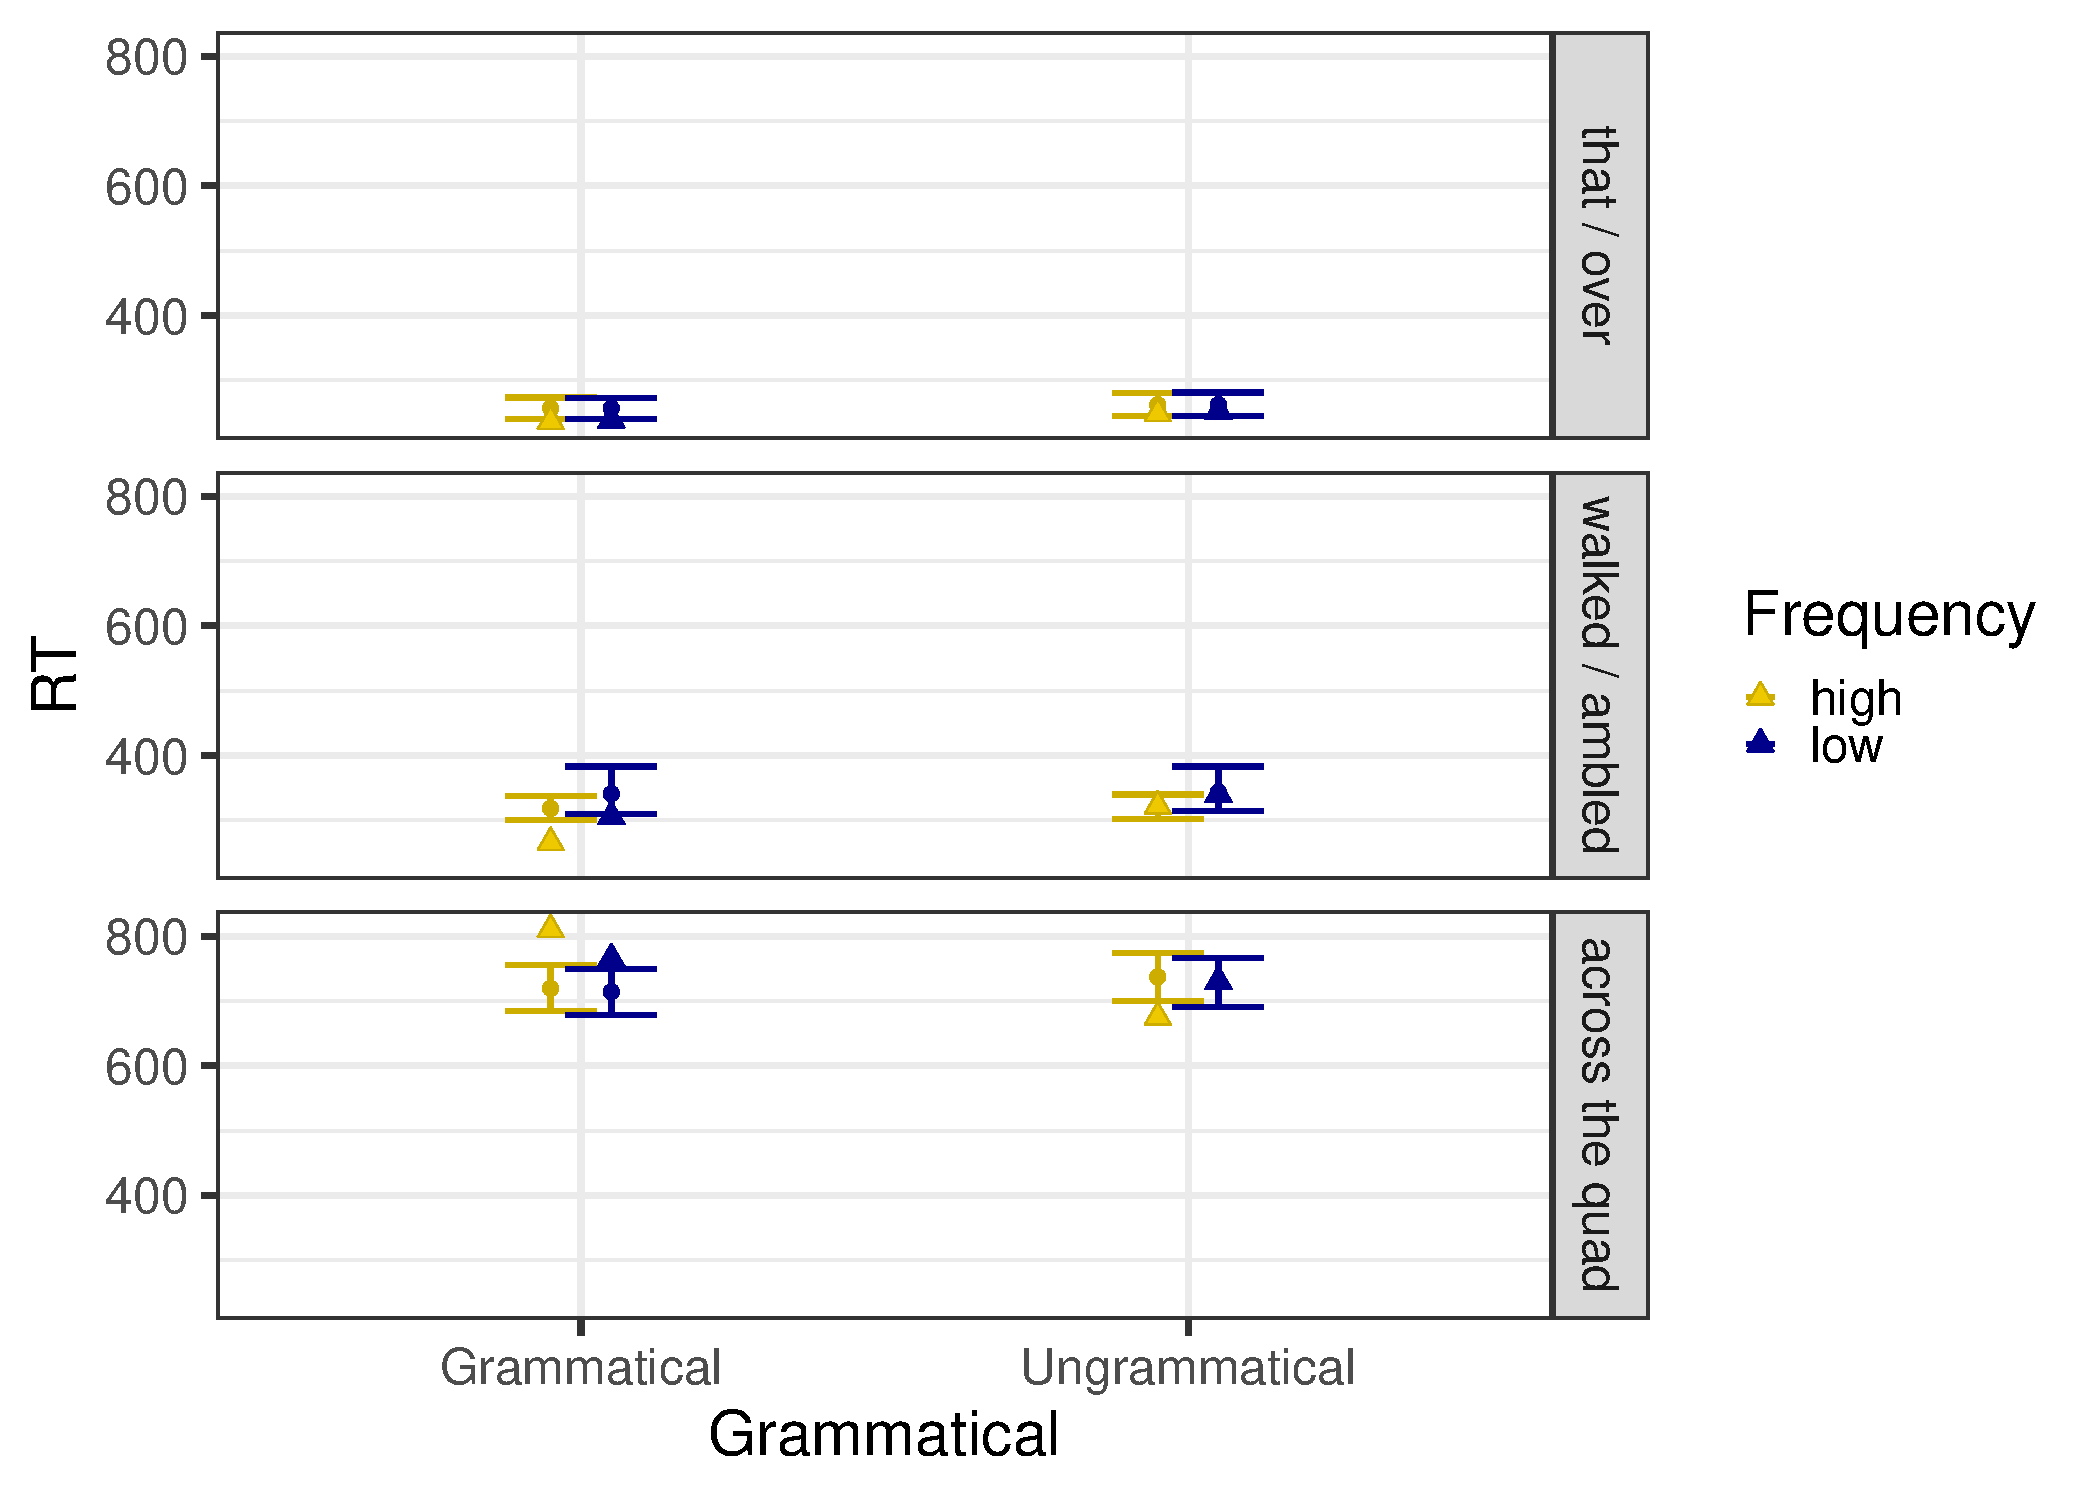
\includegraphics[width=\maxwidth]{figures/figure_staub_exp3unnamed-chunk-5-1} 

\end{knitrout}


\begin{knitrout}
\definecolor{shadecolor}{rgb}{0.969, 0.969, 0.969}\color{fgcolor}\begin{kframe}
\begin{alltt}
\hlkwd{ggsave}\hlstd{(}\hlstr{"staub-firstpass.pdf"}\hlstd{,} \hlkwc{width} \hlstd{=} \hlnum{20}\hlstd{,} \hlkwc{height} \hlstd{=} \hlnum{15}\hlstd{)}
\end{alltt}
\end{kframe}
\end{knitrout}

\begin{knitrout}
\definecolor{shadecolor}{rgb}{0.969, 0.969, 0.969}\color{fgcolor}\begin{kframe}
\begin{alltt}
\hlstd{g1} \hlkwb{<-} \hlkwd{ggplot}\hlstd{(data.to.plot,} \hlkwd{aes}\hlstd{(Region, RT,} \hlkwc{color} \hlstd{= Frequency,} \hlkwc{fill} \hlstd{= Frequency))}
\hlstd{g1} \hlkwb{<-} \hlstd{g1} \hlopt{+} \hlkwd{geom_point}\hlstd{(}\hlkwc{position} \hlstd{= dodge,} \hlkwc{size} \hlstd{=} \hlkwd{I}\hlstd{(}\hlnum{3}\hlstd{))} \hlopt{+} \hlkwd{geom_errorbar}\hlstd{(}\hlkwd{aes}\hlstd{(}\hlkwc{ymin} \hlstd{= CF1,}
    \hlkwc{ymax} \hlstd{= CF2),} \hlkwc{position} \hlstd{= dodge,} \hlkwc{width} \hlstd{=} \hlnum{0.3}\hlstd{,} \hlkwc{size} \hlstd{=} \hlkwd{I}\hlstd{(}\hlnum{1.2}\hlstd{))} \hlopt{+} \hlkwd{scale_shape_manual}\hlstd{(}\hlkwc{values} \hlstd{=} \hlnum{21}\hlopt{:}\hlnum{24}\hlstd{)} \hlopt{+}
    \hlkwd{scale_color_manual}\hlstd{(}\hlkwc{values} \hlstd{=} \hlkwd{c}\hlstd{(}\hlstr{"gold3"}\hlstd{,} \hlstr{"blue4"}\hlstd{))} \hlopt{+} \hlkwd{scale_fill_manual}\hlstd{(}\hlkwc{values} \hlstd{=} \hlkwd{c}\hlstd{(}\hlstr{"gold2"}\hlstd{,}
    \hlstr{"blue4"}\hlstd{))} \hlopt{+} \hlkwd{theme_bw}\hlstd{(}\hlnum{30}\hlstd{)}  \hlcom{# + theme(legend.justification = c(0.98, 0.9), legend.position = c(0.74, 0.9)) }
\hlstd{g1} \hlkwb{<-} \hlstd{g1} \hlopt{+} \hlkwd{coord_cartesian}\hlstd{(}\hlkwc{ylim} \hlstd{=} \hlkwd{c}\hlstd{(}\hlnum{200}\hlstd{,} \hlnum{800}\hlstd{))} \hlopt{+} \hlkwd{geom_point}\hlstd{(}\hlkwd{aes}\hlstd{(}\hlkwc{x} \hlstd{= Region,}
    \hlkwc{y} \hlstd{= Observed,} \hlkwc{fill} \hlstd{= Frequency),} \hlkwc{pch} \hlstd{=} \hlnum{24}\hlstd{,} \hlkwc{position} \hlstd{= dodge,} \hlkwc{size} \hlstd{=} \hlnum{4}\hlstd{)} \hlopt{+}
    \hlkwd{facet_grid}\hlstd{(Grammatical} \hlopt{~} \hlstd{.)}
\end{alltt}
\end{kframe}
\end{knitrout}

\begin{knitrout}
\definecolor{shadecolor}{rgb}{0.969, 0.969, 0.969}\color{fgcolor}
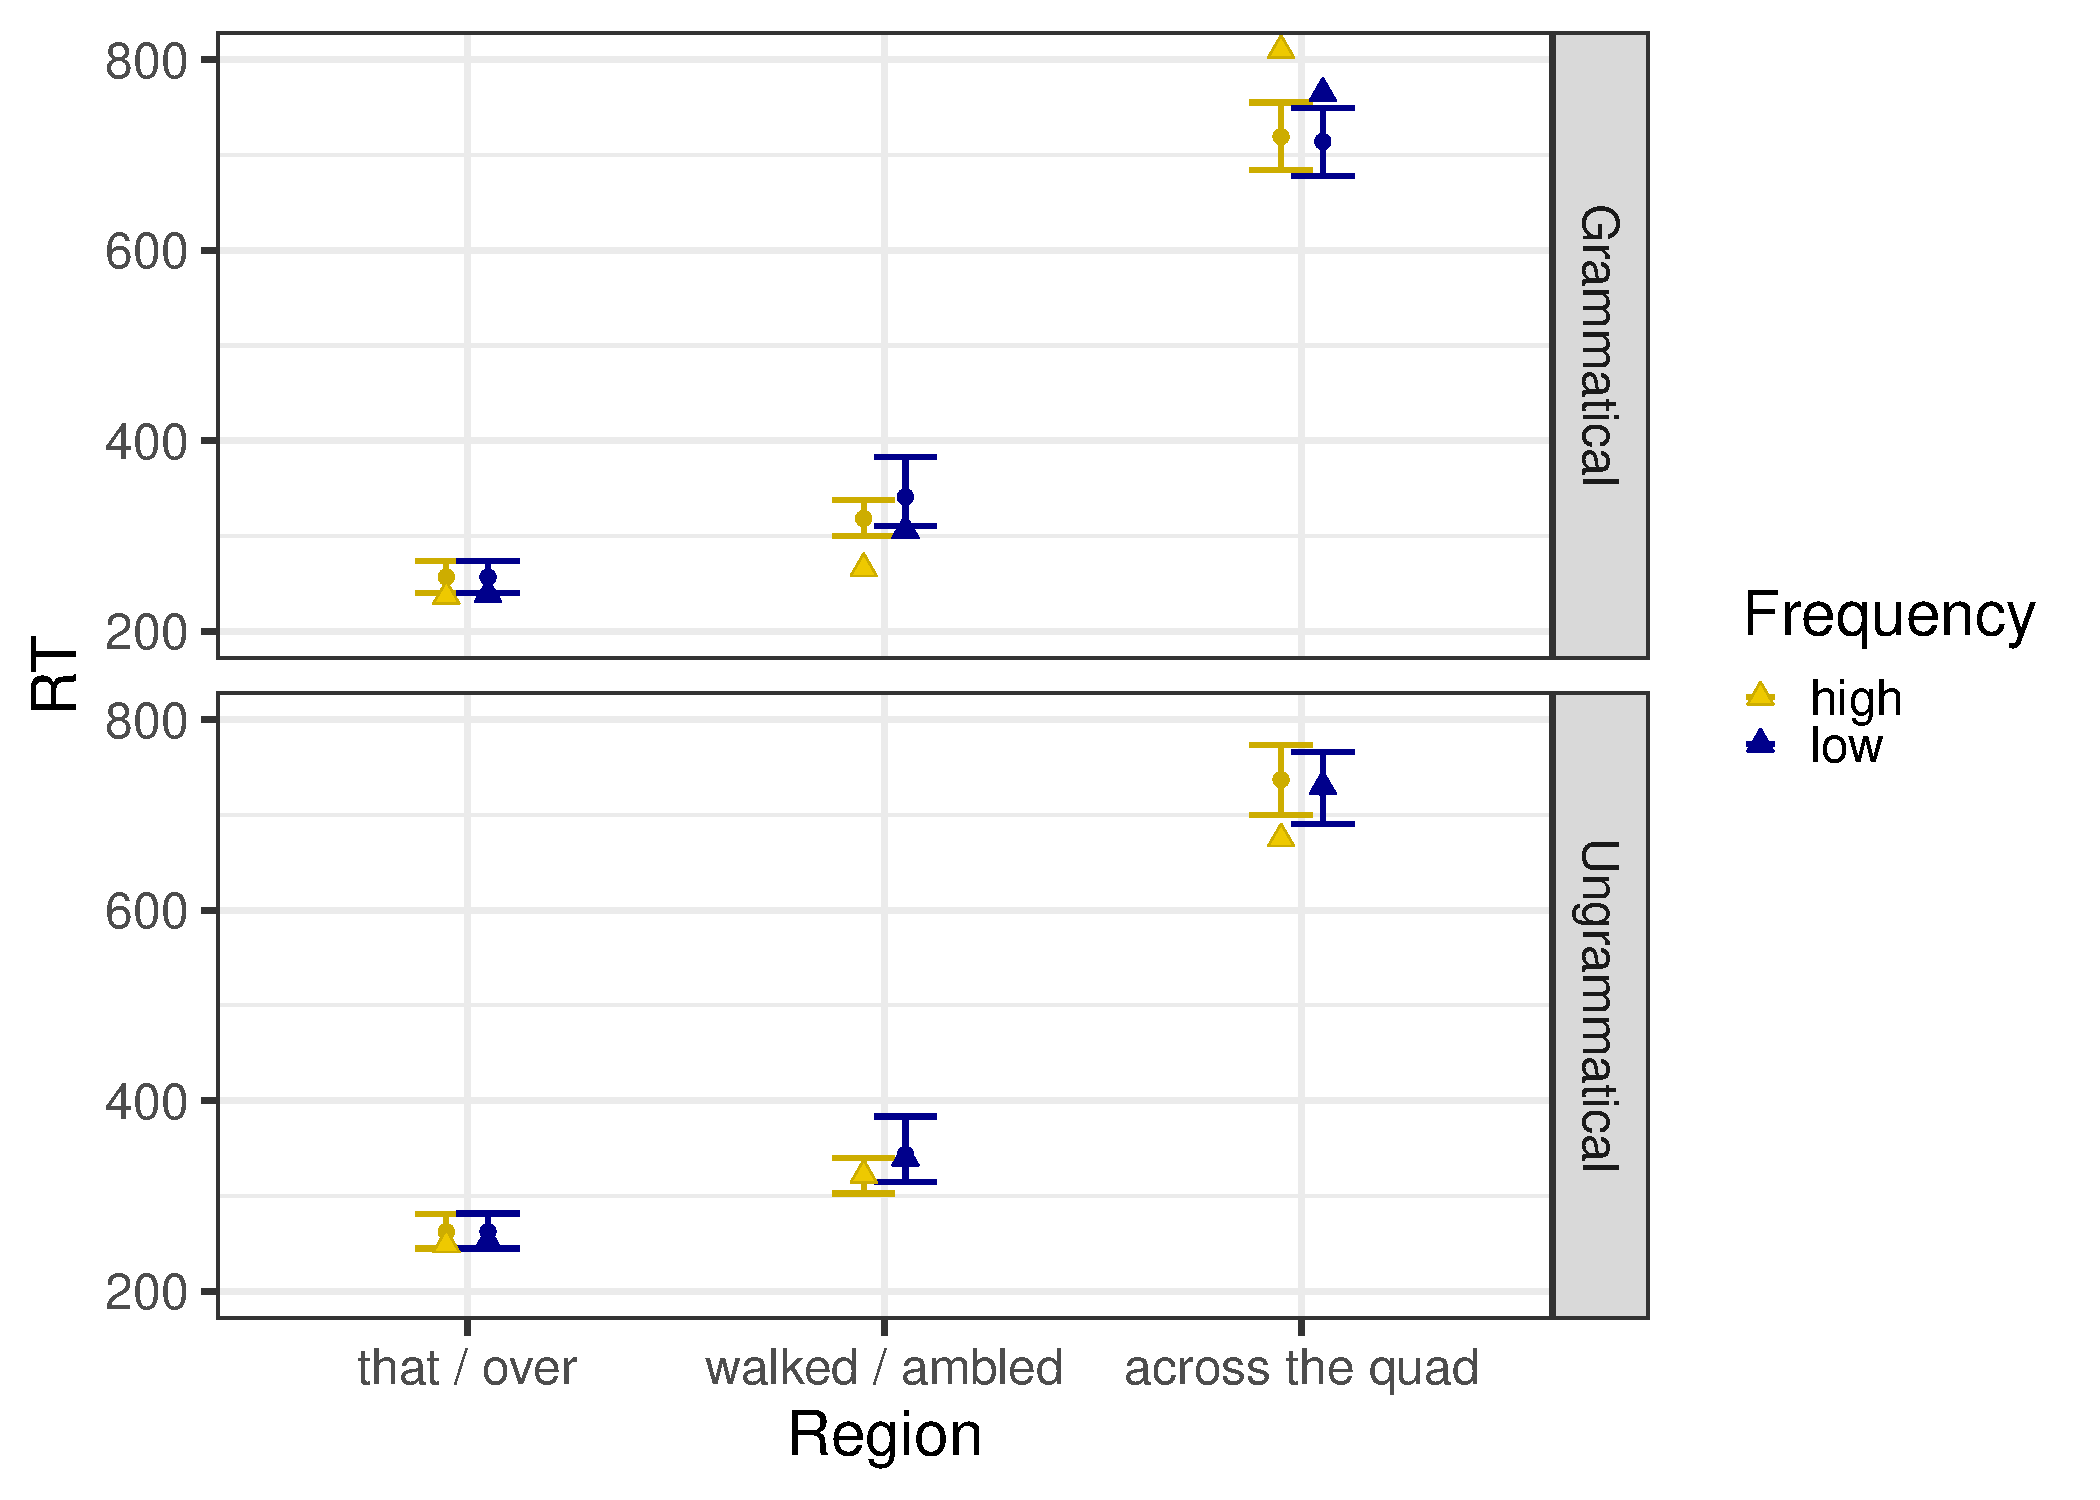
\includegraphics[width=\maxwidth]{figures/figure_staub_exp3unnamed-chunk-8-1} 

\end{knitrout}

\begin{knitrout}
\definecolor{shadecolor}{rgb}{0.969, 0.969, 0.969}\color{fgcolor}\begin{kframe}
\begin{alltt}
\hlkwd{ggsave}\hlstd{(}\hlstr{"staub-firstpass-inonegraph.pdf"}\hlstd{,} \hlkwc{width} \hlstd{=} \hlnum{20}\hlstd{,} \hlkwc{height} \hlstd{=} \hlnum{15}\hlstd{)}
\end{alltt}
\end{kframe}
\end{knitrout}

\begin{knitrout}
\definecolor{shadecolor}{rgb}{0.969, 0.969, 0.969}\color{fgcolor}\begin{kframe}
\begin{alltt}
\hlstd{ndraws} \hlkwb{<-} \hlkwd{length}\hlstd{(dataf2[,} \hlnum{1}\hlstd{])}

\hlstd{data.all} \hlkwb{<-} \hlkwd{data.frame}\hlstd{(}\hlkwc{region} \hlstd{=} \hlkwd{factor}\hlstd{(}\hlkwd{rep}\hlstd{(}\hlkwd{rep}\hlstd{(}\hlkwd{c}\hlstd{(}\hlstr{"that / over"}\hlstd{,} \hlstr{"walked / ambled"}\hlstd{,}
    \hlstr{"across the quad"}\hlstd{),} \hlkwc{each} \hlstd{= ndraws),} \hlnum{4}\hlstd{),} \hlkwc{levels} \hlstd{=} \hlkwd{c}\hlstd{(}\hlstr{"that / over"}\hlstd{,} \hlstr{"walked / ambled"}\hlstd{,}
    \hlstr{"across the quad"}\hlstd{)),} \hlkwc{grammatical} \hlstd{=} \hlkwd{c}\hlstd{(}\hlkwd{rep}\hlstd{(}\hlstr{"Grammatical"}\hlstd{, ndraws} \hlopt{*} \hlnum{6}\hlstd{),} \hlkwd{rep}\hlstd{(}\hlstr{"Ungrammatical"}\hlstd{,}
    \hlstd{ndraws} \hlopt{*} \hlnum{6}\hlstd{)),} \hlkwc{frequency} \hlstd{=} \hlkwd{c}\hlstd{(}\hlkwd{rep}\hlstd{(}\hlstr{"high"}\hlstd{, ndraws} \hlopt{*} \hlnum{3}\hlstd{),} \hlkwd{rep}\hlstd{(}\hlstr{"low"}\hlstd{, ndraws} \hlopt{*}
    \hlnum{3}\hlstd{),} \hlkwd{rep}\hlstd{(}\hlstr{"high"}\hlstd{, ndraws} \hlopt{*} \hlnum{3}\hlstd{),} \hlkwd{rep}\hlstd{(}\hlstr{"low"}\hlstd{, ndraws} \hlopt{*} \hlnum{3}\hlstd{)),} \hlkwc{Reg} \hlstd{=} \hlkwd{c}\hlstd{(dataf2[,}
    \hlnum{1}\hlstd{], dataf2[,} \hlnum{2}\hlstd{], dataf2[,} \hlnum{3}\hlstd{], dataf2[,} \hlnum{4}\hlstd{], dataf2[,} \hlnum{5}\hlstd{], dataf2[,} \hlnum{6}\hlstd{], dataf2[,}
    \hlnum{7}\hlstd{], dataf2[,} \hlnum{8}\hlstd{], dataf2[,} \hlnum{9}\hlstd{], dataf2[,} \hlnum{10}\hlstd{], dataf2[,} \hlnum{11}\hlstd{], dataf2[,} \hlnum{12}\hlstd{]),}
    \hlkwc{x} \hlstd{=} \hlkwd{rep}\hlstd{(}\hlkwd{c}\hlstd{(}\hlnum{0.06}\hlstd{,} \hlnum{0.13}\hlstd{,} \hlnum{0.4}\hlstd{,} \hlnum{0.07}\hlstd{,} \hlnum{0.17}\hlstd{,} \hlnum{0.46}\hlstd{,} \hlnum{0.16}\hlstd{,} \hlnum{0.29}\hlstd{,} \hlnum{0.59}\hlstd{,} \hlnum{0.12}\hlstd{,} \hlnum{0.34}\hlstd{,}
        \hlnum{0.52}\hlstd{),} \hlkwc{each} \hlstd{= ndraws))}

\hlkwd{str}\hlstd{(data.all)}
\end{alltt}
\begin{verbatim}
## 'data.frame':	67056 obs. of  5 variables:
##  $ region     : Factor w/ 3 levels "that / over",..: 1 1 1 1 1 1 1 1 1 1 ...
##  $ grammatical: Factor w/ 2 levels "Grammatical",..: 1 1 1 1 1 1 1 1 1 1 ...
##  $ frequency  : Factor w/ 2 levels "high","low": 1 1 1 1 1 1 1 1 1 1 ...
##  $ Reg        : num  0.0318 0.0318 0.0318 0.0341 0.0341 ...
##  $ x          : num  0.06 0.06 0.06 0.06 0.06 0.06 0.06 0.06 0.06 0.06 ...
\end{verbatim}
\begin{alltt}
\hlcom{# data.all <- subset(data.all, RT > 50 & RT < 3000)}

\hlkwd{library}\hlstd{(ggplot2)}

\hlkwd{library}\hlstd{(dplyr)}

\hlstd{data.to.plot} \hlkwb{<-} \hlstd{data.all} \hlopt \hlkwd{group_by}\hlstd{(region, grammatical, frequency)} \hlopt \hlkwd{summarise}\hlstd{(}\hlkwc{Region} \hlstd{=} \hlkwd{first}\hlstd{(region),}
    \hlkwc{Grammatical} \hlstd{=} \hlkwd{first}\hlstd{(grammatical),} \hlkwc{Frequency} \hlstd{=} \hlkwd{first}\hlstd{(frequency),} \hlkwc{CF1} \hlstd{=} \hlkwd{quantile}\hlstd{(Reg,}
        \hlkwc{probs} \hlstd{=} \hlkwd{c}\hlstd{(}\hlnum{0.05}\hlstd{,} \hlnum{0.95}\hlstd{))[}\hlnum{1}\hlstd{],} \hlkwc{CF2} \hlstd{=} \hlkwd{quantile}\hlstd{(Reg,} \hlkwc{probs} \hlstd{=} \hlkwd{c}\hlstd{(}\hlnum{0.05}\hlstd{,} \hlnum{0.95}\hlstd{))[}\hlnum{2}\hlstd{],}
    \hlkwc{Regressions} \hlstd{=} \hlkwd{mean}\hlstd{(Reg),} \hlkwc{Observed} \hlstd{=} \hlkwd{first}\hlstd{(x))}
\end{alltt}


{\ttfamily\noindent\itshape\color{messagecolor}{\#\# `summarise()` has grouped output by 'region', 'grammatical'. You can override using the `.groups` argument.}}\begin{alltt}
\hlstd{data.to.plot}
\end{alltt}
\begin{verbatim}
## # A tibble: 12 x 10
## # Groups:   region, grammatical [6]
##    region grammatical frequency Region Grammatical Frequency    CF1    CF2
##    <fct>  <fct>       <fct>     <fct>  <fct>       <fct>      <dbl>  <dbl>
##  1 that ~ Grammatical high      that ~ Grammatical high      0.0282 0.0695
##  2 that ~ Grammatical low       that ~ Grammatical low       0.0152 0.0427
##  3 that ~ Ungrammati~ high      that ~ Ungrammati~ high      0.153  0.247 
##  4 that ~ Ungrammati~ low       that ~ Ungrammati~ low       0.203  0.301 
##  5 walke~ Grammatical high      walke~ Grammatical high      0.0469 0.0672
##  6 walke~ Grammatical low       walke~ Grammatical low       0.0471 0.0673
##  7 walke~ Ungrammati~ high      walke~ Ungrammati~ high      0.230  0.319 
##  8 walke~ Ungrammati~ low       walke~ Ungrammati~ low       0.262  0.340 
##  9 acros~ Grammatical high      acros~ Grammatical high      0.420  0.516 
## 10 acros~ Grammatical low       acros~ Grammatical low       0.431  0.518 
## 11 acros~ Ungrammati~ high      acros~ Ungrammati~ high      0.438  0.516 
## 12 acros~ Ungrammati~ low       acros~ Ungrammati~ low       0.476  0.562 
## # ... with 2 more variables: Regressions <dbl>, Observed <dbl>
\end{verbatim}
\begin{alltt}
\hlstd{g1} \hlkwb{<-} \hlkwd{ggplot}\hlstd{(data.to.plot,} \hlkwd{aes}\hlstd{(Grammatical, Regressions,} \hlkwc{color} \hlstd{= Frequency,}
    \hlkwc{fill} \hlstd{= Frequency))}
\hlstd{g1} \hlkwb{<-} \hlstd{g1} \hlopt{+} \hlkwd{geom_point}\hlstd{(}\hlkwc{position} \hlstd{= dodge,} \hlkwc{size} \hlstd{=} \hlkwd{I}\hlstd{(}\hlnum{3}\hlstd{))} \hlopt{+} \hlkwd{geom_errorbar}\hlstd{(}\hlkwd{aes}\hlstd{(}\hlkwc{ymin} \hlstd{= CF1,}
    \hlkwc{ymax} \hlstd{= CF2),} \hlkwc{position} \hlstd{= dodge,} \hlkwc{width} \hlstd{=} \hlnum{0.3}\hlstd{,} \hlkwc{size} \hlstd{=} \hlkwd{I}\hlstd{(}\hlnum{1.2}\hlstd{))} \hlopt{+} \hlkwd{scale_shape_manual}\hlstd{(}\hlkwc{values} \hlstd{=} \hlnum{21}\hlopt{:}\hlnum{24}\hlstd{)} \hlopt{+}
    \hlkwd{scale_color_manual}\hlstd{(}\hlkwc{values} \hlstd{=} \hlkwd{c}\hlstd{(}\hlstr{"gold3"}\hlstd{,} \hlstr{"blue4"}\hlstd{))} \hlopt{+} \hlkwd{scale_fill_manual}\hlstd{(}\hlkwc{values} \hlstd{=} \hlkwd{c}\hlstd{(}\hlstr{"gold2"}\hlstd{,}
    \hlstr{"blue4"}\hlstd{))} \hlopt{+} \hlkwd{theme_bw}\hlstd{(}\hlnum{30}\hlstd{)}  \hlcom{# + theme(legend.justification = c(0.98, 0.9), legend.position = c(0.74, 0.9)) }
\hlstd{g1} \hlkwb{<-} \hlstd{g1} \hlopt{+} \hlkwd{geom_point}\hlstd{(}\hlkwd{aes}\hlstd{(}\hlkwc{x} \hlstd{= Grammatical,} \hlkwc{y} \hlstd{= Observed,} \hlkwc{fill} \hlstd{= Frequency),}
    \hlkwc{pch} \hlstd{=} \hlnum{24}\hlstd{,} \hlkwc{position} \hlstd{= dodge,} \hlkwc{size} \hlstd{=} \hlnum{4}\hlstd{)} \hlopt{+} \hlkwd{facet_grid}\hlstd{(Region} \hlopt{~} \hlstd{.)}
\end{alltt}
\end{kframe}
\end{knitrout}

\begin{knitrout}
\definecolor{shadecolor}{rgb}{0.969, 0.969, 0.969}\color{fgcolor}
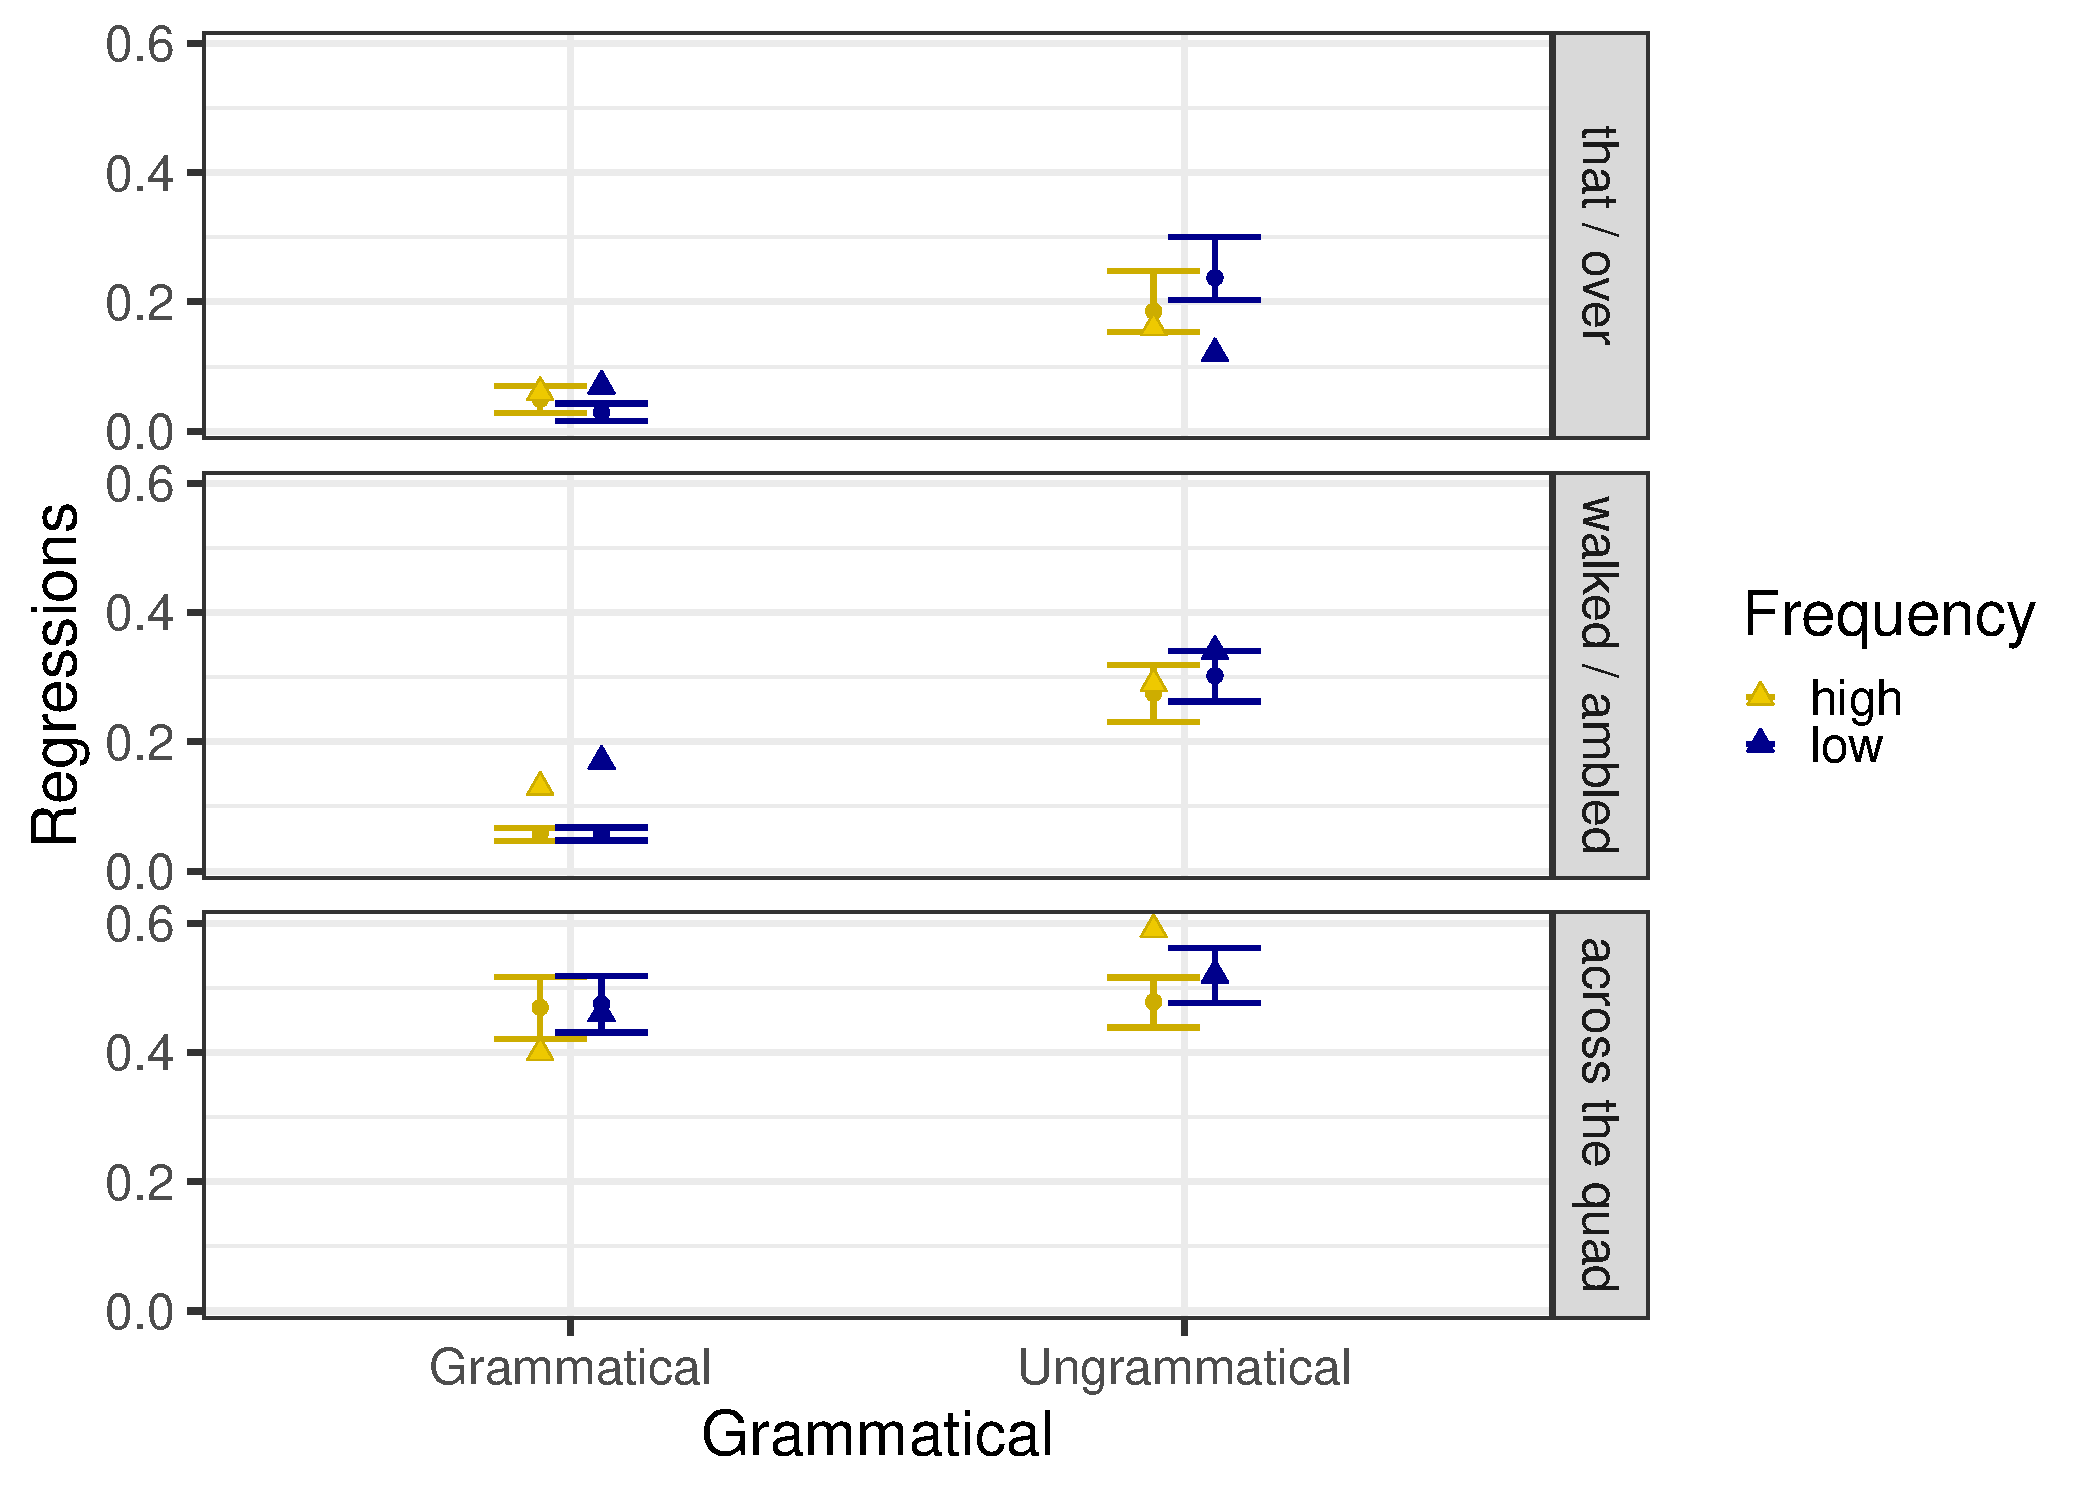
\includegraphics[width=\maxwidth]{figures/figure_staub_exp3unnamed-chunk-11-1} 

\end{knitrout}


\begin{knitrout}
\definecolor{shadecolor}{rgb}{0.969, 0.969, 0.969}\color{fgcolor}\begin{kframe}
\begin{alltt}
\hlkwd{ggsave}\hlstd{(}\hlstr{"staub-regressions.pdf"}\hlstd{,} \hlkwc{width} \hlstd{=} \hlnum{20}\hlstd{,} \hlkwc{height} \hlstd{=} \hlnum{15}\hlstd{)}
\end{alltt}
\end{kframe}
\end{knitrout}

\begin{knitrout}
\definecolor{shadecolor}{rgb}{0.969, 0.969, 0.969}\color{fgcolor}\begin{kframe}
\begin{alltt}
\hlstd{g1} \hlkwb{<-} \hlkwd{ggplot}\hlstd{(data.to.plot,} \hlkwd{aes}\hlstd{(Region, Regressions,} \hlkwc{color} \hlstd{= Frequency,} \hlkwc{fill} \hlstd{= Frequency))}
\hlstd{g1} \hlkwb{<-} \hlstd{g1} \hlopt{+} \hlkwd{geom_point}\hlstd{(}\hlkwc{position} \hlstd{= dodge,} \hlkwc{size} \hlstd{=} \hlkwd{I}\hlstd{(}\hlnum{3}\hlstd{))} \hlopt{+} \hlkwd{geom_errorbar}\hlstd{(}\hlkwd{aes}\hlstd{(}\hlkwc{ymin} \hlstd{= CF1,}
    \hlkwc{ymax} \hlstd{= CF2),} \hlkwc{position} \hlstd{= dodge,} \hlkwc{width} \hlstd{=} \hlnum{0.3}\hlstd{,} \hlkwc{size} \hlstd{=} \hlkwd{I}\hlstd{(}\hlnum{1.2}\hlstd{))} \hlopt{+} \hlkwd{scale_shape_manual}\hlstd{(}\hlkwc{values} \hlstd{=} \hlnum{21}\hlopt{:}\hlnum{24}\hlstd{)} \hlopt{+}
    \hlkwd{scale_color_manual}\hlstd{(}\hlkwc{values} \hlstd{=} \hlkwd{c}\hlstd{(}\hlstr{"gold3"}\hlstd{,} \hlstr{"blue4"}\hlstd{))} \hlopt{+} \hlkwd{scale_fill_manual}\hlstd{(}\hlkwc{values} \hlstd{=} \hlkwd{c}\hlstd{(}\hlstr{"gold2"}\hlstd{,}
    \hlstr{"blue4"}\hlstd{))} \hlopt{+} \hlkwd{theme_bw}\hlstd{(}\hlnum{30}\hlstd{)}  \hlcom{# + theme(legend.justification = c(0.98, 0.9), legend.position = c(0.74, 0.9)) }
\hlstd{g1} \hlkwb{<-} \hlstd{g1} \hlopt{+} \hlkwd{coord_cartesian}\hlstd{(}\hlkwc{ylim} \hlstd{=} \hlkwd{c}\hlstd{(}\hlnum{0}\hlstd{,} \hlnum{0.7}\hlstd{))} \hlopt{+} \hlkwd{geom_point}\hlstd{(}\hlkwd{aes}\hlstd{(}\hlkwc{x} \hlstd{= Region,} \hlkwc{y} \hlstd{= Observed,}
    \hlkwc{fill} \hlstd{= Frequency),} \hlkwc{pch} \hlstd{=} \hlnum{24}\hlstd{,} \hlkwc{position} \hlstd{= dodge,} \hlkwc{size} \hlstd{=} \hlnum{4}\hlstd{)} \hlopt{+} \hlkwd{facet_grid}\hlstd{(Grammatical} \hlopt{~}
    \hlstd{.)}
\end{alltt}
\end{kframe}
\end{knitrout}

\begin{knitrout}
\definecolor{shadecolor}{rgb}{0.969, 0.969, 0.969}\color{fgcolor}
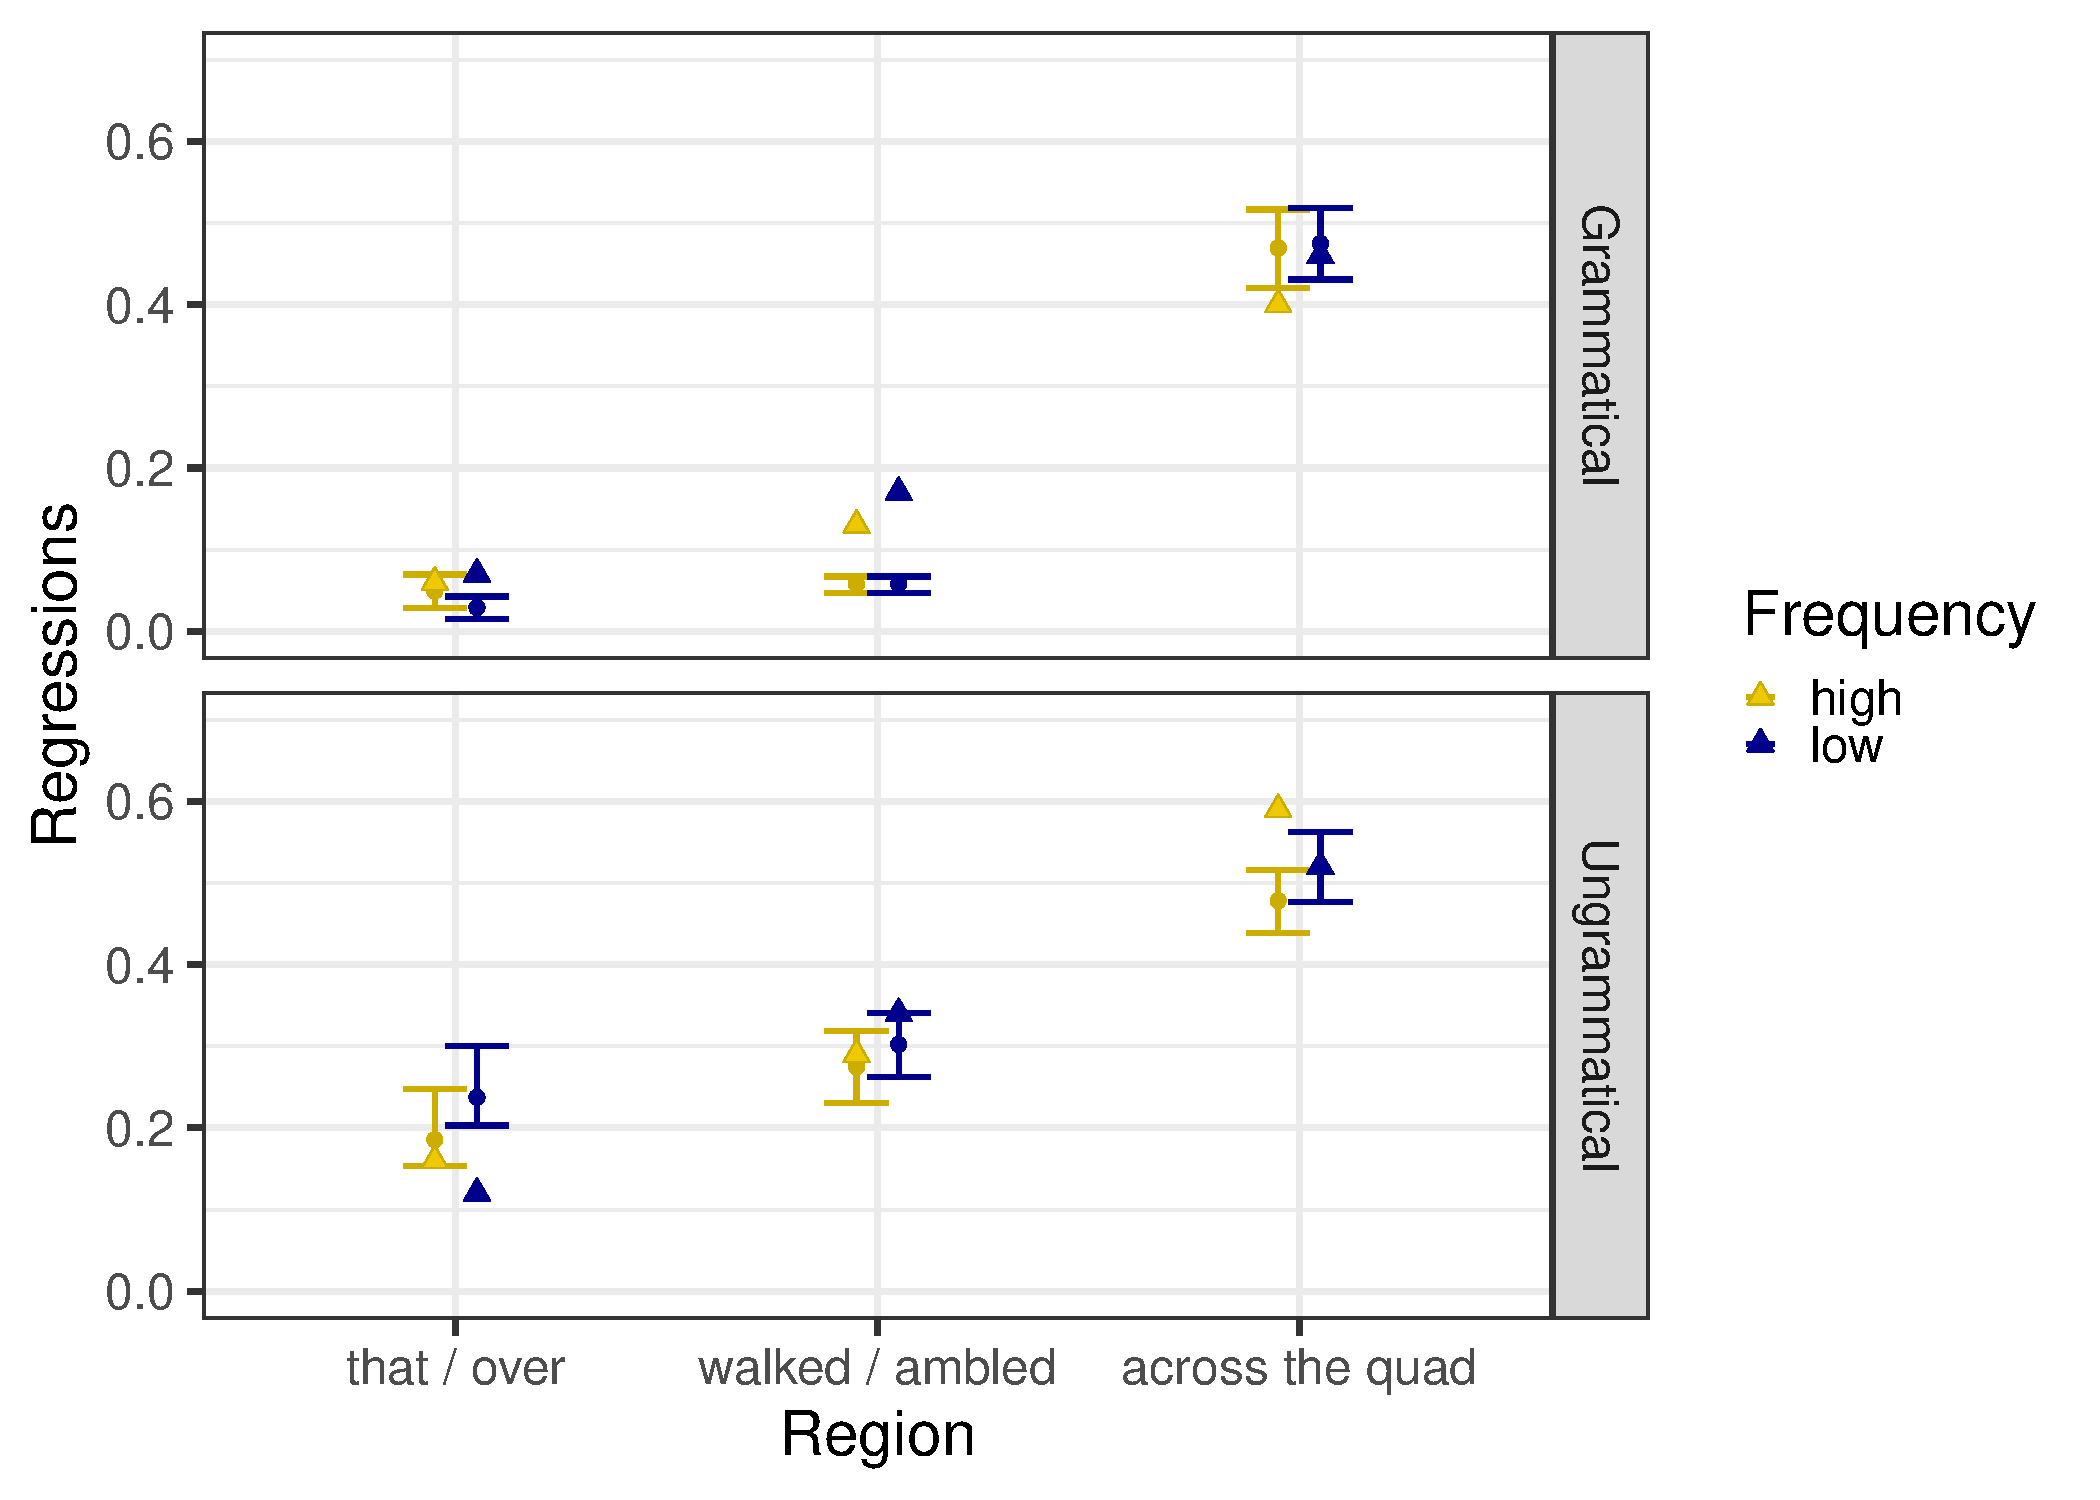
\includegraphics[width=\maxwidth]{figures/figure_staub_exp3unnamed-chunk-14-1} 

\end{knitrout}
\begin{knitrout}
\definecolor{shadecolor}{rgb}{0.969, 0.969, 0.969}\color{fgcolor}\begin{kframe}
\begin{alltt}
\hlkwd{ggsave}\hlstd{(}\hlstr{"staub-regressions-inonegraph.pdf"}\hlstd{,} \hlkwc{width} \hlstd{=} \hlnum{20}\hlstd{,} \hlkwc{height} \hlstd{=} \hlnum{15}\hlstd{)}
\end{alltt}
\end{kframe}
\end{knitrout}


\section{Parameters}



\subsection{LF}

\begin{knitrout}
\definecolor{shadecolor}{rgb}{0.969, 0.969, 0.969}\color{fgcolor}\begin{kframe}
\begin{alltt}
\hlcom{############# PARAMS###########}
\hlstd{draws} \hlkwb{<-} \hlkwd{createdraws}\hlstd{(}\hlstr{"lf"}\hlstd{)}
\end{alltt}


{\ttfamily\noindent\itshape\color{messagecolor}{\#\# Note: Using an external vector in selections is ambiguous.\\\#\# i Use `all\_of(param)` instead of `param` to silence this message.\\\#\# i See <https://tidyselect.r-lib.org/reference/faq-external-vector.html>.\\\#\# This message is displayed once per session.}}\begin{alltt}
\hlkwd{str}\hlstd{(draws)}
\end{alltt}
\begin{verbatim}
##  num [1:2794, 1:2] 0.0556 0.0556 0.0404 0.0483 0.0483 ...
\end{verbatim}
\begin{alltt}
\hlkwd{Rhat}\hlstd{(draws)}
\end{alltt}
\begin{verbatim}
## [1] 1.011642
\end{verbatim}
\end{kframe}
\end{knitrout}

Mean etc.

\begin{knitrout}
\definecolor{shadecolor}{rgb}{0.969, 0.969, 0.969}\color{fgcolor}\begin{kframe}
\begin{alltt}
\hlkwd{tail}\hlstd{(draws)}
\end{alltt}
\begin{verbatim}
##               [,1]       [,2]
## [2789,] 0.05125586 0.04595704
## [2790,] 0.05125586 0.04595704
## [2791,] 0.05125586 0.04595704
## [2792,] 0.05551180 0.04595704
## [2793,] 0.05551180 0.04595704
## [2794,] 0.05551180 0.04595704
\end{verbatim}
\begin{alltt}
\hlkwd{mean}\hlstd{(}\hlkwd{c}\hlstd{(draws[,} \hlnum{1}\hlopt{:}\hlnum{2}\hlstd{]))}
\end{alltt}
\begin{verbatim}
## [1] 0.0524086
\end{verbatim}
\begin{alltt}
\hlkwd{median}\hlstd{(}\hlkwd{c}\hlstd{(draws[,} \hlnum{1}\hlopt{:}\hlnum{2}\hlstd{]))}
\end{alltt}
\begin{verbatim}
## [1] 0.05165914
\end{verbatim}
\begin{alltt}
\hlkwd{sd}\hlstd{(}\hlkwd{c}\hlstd{(draws[,} \hlnum{1}\hlopt{:}\hlnum{2}\hlstd{]))}
\end{alltt}
\begin{verbatim}
## [1] 0.009714798
\end{verbatim}
\begin{alltt}
\hlstd{g1} \hlkwb{<-} \hlkwd{ggplot}\hlstd{(}\hlkwd{data.frame}\hlstd{(}\hlkwc{latency_factor} \hlstd{=} \hlkwd{c}\hlstd{(draws[,} \hlnum{1}\hlopt{:}\hlnum{2}\hlstd{])),} \hlkwd{aes}\hlstd{(latency_factor))}
\hlstd{g1} \hlkwb{<-} \hlstd{g1} \hlopt{+} \hlkwd{geom_histogram}\hlstd{()} \hlopt{+} \hlkwd{theme_bw}\hlstd{(}\hlnum{28}\hlstd{)}
\hlstd{g1}
\end{alltt}


{\ttfamily\noindent\itshape\color{messagecolor}{\#\# `stat\_bin()` using `bins = 30`. Pick better value with `binwidth`.}}\end{kframe}
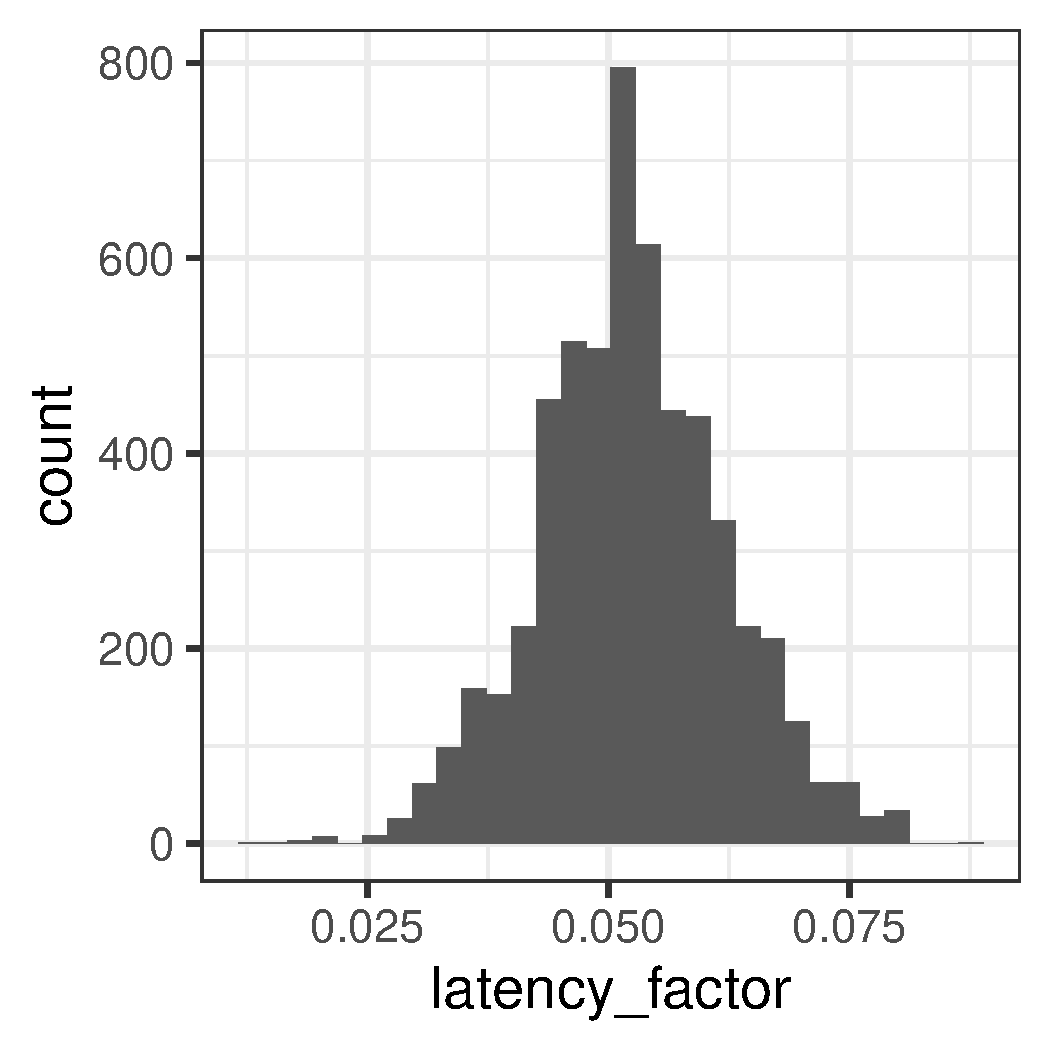
\includegraphics[width=\maxwidth]{figures/figure_staub_exp3unnamed-chunk-18-1} 
\begin{kframe}\begin{alltt}
\hlkwd{ggsave}\hlstd{(}\hlstr{"staub-lf.pdf"}\hlstd{,} \hlkwc{width} \hlstd{=} \hlnum{20}\hlstd{,} \hlkwc{height} \hlstd{=} \hlnum{12}\hlstd{)}
\end{alltt}


{\ttfamily\noindent\itshape\color{messagecolor}{\#\# `stat\_bin()` using `bins = 30`. Pick better value with `binwidth`.}}\end{kframe}
\end{knitrout}

\subsection{LE}

\begin{knitrout}
\definecolor{shadecolor}{rgb}{0.969, 0.969, 0.969}\color{fgcolor}\begin{kframe}
\begin{alltt}
\hlcom{############# PARAMS###########}
\hlstd{draws} \hlkwb{<-} \hlkwd{createdraws}\hlstd{(}\hlstr{"le"}\hlstd{)}

\hlkwd{str}\hlstd{(draws)}
\end{alltt}
\begin{verbatim}
##  num [1:2794, 1:2] 0.1 0.1 0.1 0.131 0.131 ...
\end{verbatim}
\begin{alltt}
\hlkwd{Rhat}\hlstd{(draws)}
\end{alltt}
\begin{verbatim}
## [1] 1.002964
\end{verbatim}
\end{kframe}
\end{knitrout}

Mean etc.

\begin{knitrout}
\definecolor{shadecolor}{rgb}{0.969, 0.969, 0.969}\color{fgcolor}\begin{kframe}
\begin{alltt}
\hlkwd{tail}\hlstd{(draws)}
\end{alltt}
\begin{verbatim}
##              [,1]       [,2]
## [2789,] 0.1217190 0.07315806
## [2790,] 0.1566882 0.09953382
## [2791,] 0.1220705 0.09953382
## [2792,] 0.1220705 0.09953382
## [2793,] 0.1220705 0.09953382
## [2794,] 0.1220705 0.09953382
\end{verbatim}
\begin{alltt}
\hlkwd{mean}\hlstd{(}\hlkwd{c}\hlstd{(draws[,} \hlnum{1}\hlopt{:}\hlnum{2}\hlstd{]))}
\end{alltt}
\begin{verbatim}
## [1] 0.1119095
\end{verbatim}
\begin{alltt}
\hlkwd{median}\hlstd{(}\hlkwd{c}\hlstd{(draws[,} \hlnum{1}\hlopt{:}\hlnum{2}\hlstd{]))}
\end{alltt}
\begin{verbatim}
## [1] 0.1031822
\end{verbatim}
\begin{alltt}
\hlkwd{sd}\hlstd{(}\hlkwd{c}\hlstd{(draws[,} \hlnum{1}\hlopt{:}\hlnum{2}\hlstd{]))}
\end{alltt}
\begin{verbatim}
## [1] 0.05774515
\end{verbatim}
\begin{alltt}
\hlstd{g1} \hlkwb{<-} \hlkwd{ggplot}\hlstd{(}\hlkwd{data.frame}\hlstd{(}\hlkwc{latency_exponent} \hlstd{=} \hlkwd{c}\hlstd{(draws[,} \hlnum{1}\hlopt{:}\hlnum{2}\hlstd{])),} \hlkwd{aes}\hlstd{(latency_exponent))}
\hlstd{g1} \hlkwb{<-} \hlstd{g1} \hlopt{+} \hlkwd{geom_histogram}\hlstd{()} \hlopt{+} \hlkwd{theme_bw}\hlstd{(}\hlnum{28}\hlstd{)}
\hlstd{g1}
\end{alltt}


{\ttfamily\noindent\itshape\color{messagecolor}{\#\# `stat\_bin()` using `bins = 30`. Pick better value with `binwidth`.}}\end{kframe}
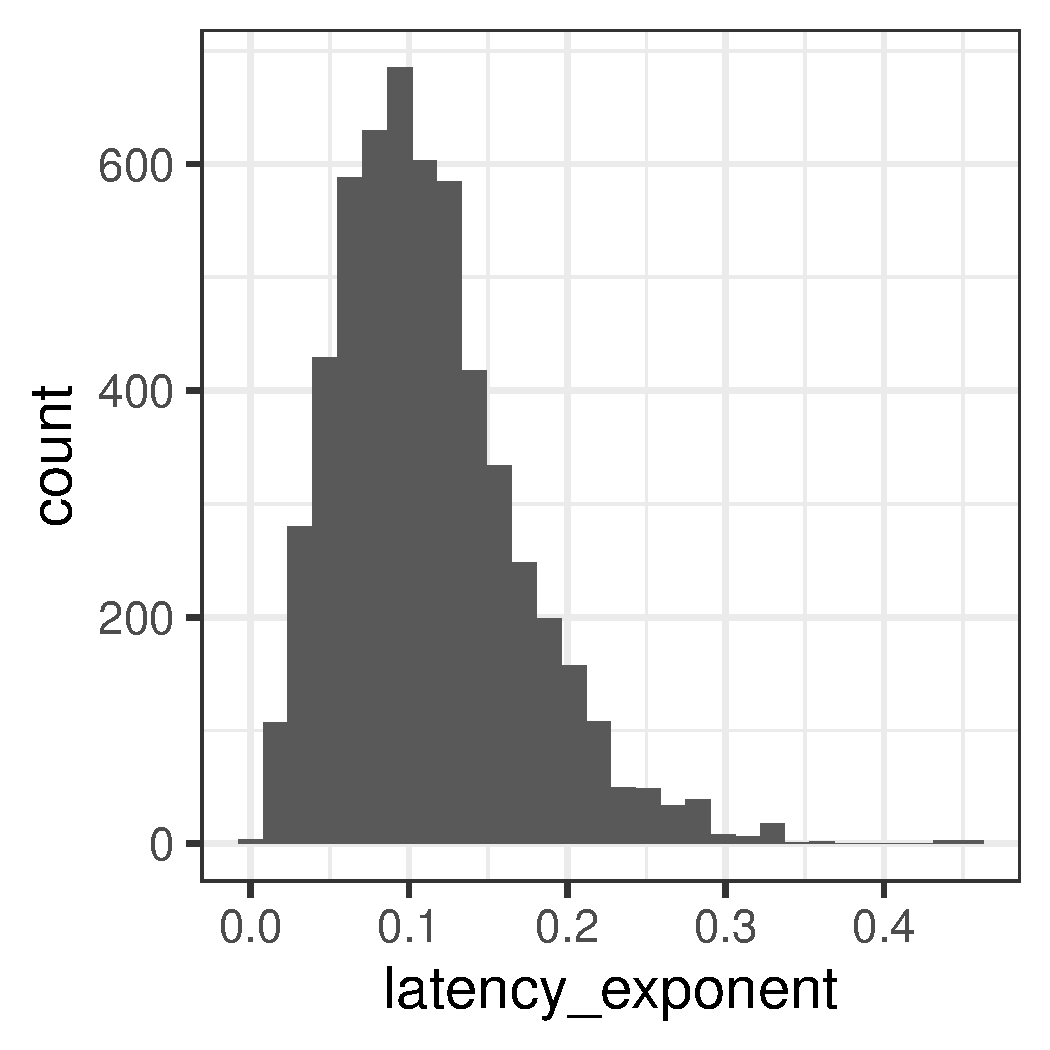
\includegraphics[width=\maxwidth]{figures/figure_staub_exp3unnamed-chunk-20-1} 
\begin{kframe}\begin{alltt}
\hlkwd{ggsave}\hlstd{(}\hlstr{"staub-le.pdf"}\hlstd{,} \hlkwc{width} \hlstd{=} \hlnum{20}\hlstd{,} \hlkwc{height} \hlstd{=} \hlnum{12}\hlstd{)}
\end{alltt}


{\ttfamily\noindent\itshape\color{messagecolor}{\#\# `stat\_bin()` using `bins = 30`. Pick better value with `binwidth`.}}\end{kframe}
\end{knitrout}

\subsection{Emma preparation time}

\begin{knitrout}
\definecolor{shadecolor}{rgb}{0.969, 0.969, 0.969}\color{fgcolor}\begin{kframe}
\begin{alltt}
\hlcom{############# PARAMS###########}
\hlstd{draws} \hlkwb{<-} \hlkwd{createdraws}\hlstd{(}\hlstr{"emma_prep_time"}\hlstd{)}

\hlkwd{str}\hlstd{(draws)}
\end{alltt}
\begin{verbatim}
##  num [1:2794, 1:2] 0.00924 0.00407 0.00407 0.00428 0.00689 ...
\end{verbatim}
\begin{alltt}
\hlkwd{Rhat}\hlstd{(draws)}
\end{alltt}
\begin{verbatim}
## [1] 1.021713
\end{verbatim}
\end{kframe}
\end{knitrout}

Mean etc.

\begin{knitrout}
\definecolor{shadecolor}{rgb}{0.969, 0.969, 0.969}\color{fgcolor}\begin{kframe}
\begin{alltt}
\hlkwd{tail}\hlstd{(draws)}
\end{alltt}
\begin{verbatim}
##                [,1]         [,2]
## [2789,] 0.004869950 0.0006885783
## [2790,] 0.003709092 0.0006885783
## [2791,] 0.003709092 0.0006885783
## [2792,] 0.005699268 0.0046673239
## [2793,] 0.005699268 0.0046673239
## [2794,] 0.005699268 0.0046673239
\end{verbatim}
\begin{alltt}
\hlkwd{mean}\hlstd{(}\hlkwd{c}\hlstd{(draws[,} \hlnum{1}\hlopt{:}\hlnum{2}\hlstd{]))}
\end{alltt}
\begin{verbatim}
## [1] 0.01054056
\end{verbatim}
\begin{alltt}
\hlkwd{median}\hlstd{(}\hlkwd{c}\hlstd{(draws[,} \hlnum{1}\hlopt{:}\hlnum{2}\hlstd{]))}
\end{alltt}
\begin{verbatim}
## [1] 0.005892357
\end{verbatim}
\begin{alltt}
\hlkwd{sd}\hlstd{(}\hlkwd{c}\hlstd{(draws[,} \hlnum{1}\hlopt{:}\hlnum{2}\hlstd{]))}
\end{alltt}
\begin{verbatim}
## [1] 0.02030516
\end{verbatim}
\begin{alltt}
\hlstd{g1} \hlkwb{<-} \hlkwd{ggplot}\hlstd{(}\hlkwd{data.frame}\hlstd{(}\hlkwc{emma_prep_time} \hlstd{=} \hlkwd{c}\hlstd{(draws[,} \hlnum{1}\hlopt{:}\hlnum{2}\hlstd{])),} \hlkwd{aes}\hlstd{(emma_prep_time))}
\hlstd{g1} \hlkwb{<-} \hlstd{g1} \hlopt{+} \hlkwd{geom_histogram}\hlstd{(}\hlkwc{xlim} \hlstd{=} \hlkwd{c}\hlstd{(}\hlnum{0}\hlstd{,} \hlnum{0.05}\hlstd{))} \hlopt{+} \hlkwd{theme_bw}\hlstd{(}\hlnum{28}\hlstd{)}
\end{alltt}


{\ttfamily\noindent\color{warningcolor}{\#\# Warning: Ignoring unknown parameters: xlim}}\begin{alltt}
\hlstd{g1}
\end{alltt}


{\ttfamily\noindent\itshape\color{messagecolor}{\#\# `stat\_bin()` using `bins = 30`. Pick better value with `binwidth`.}}\end{kframe}
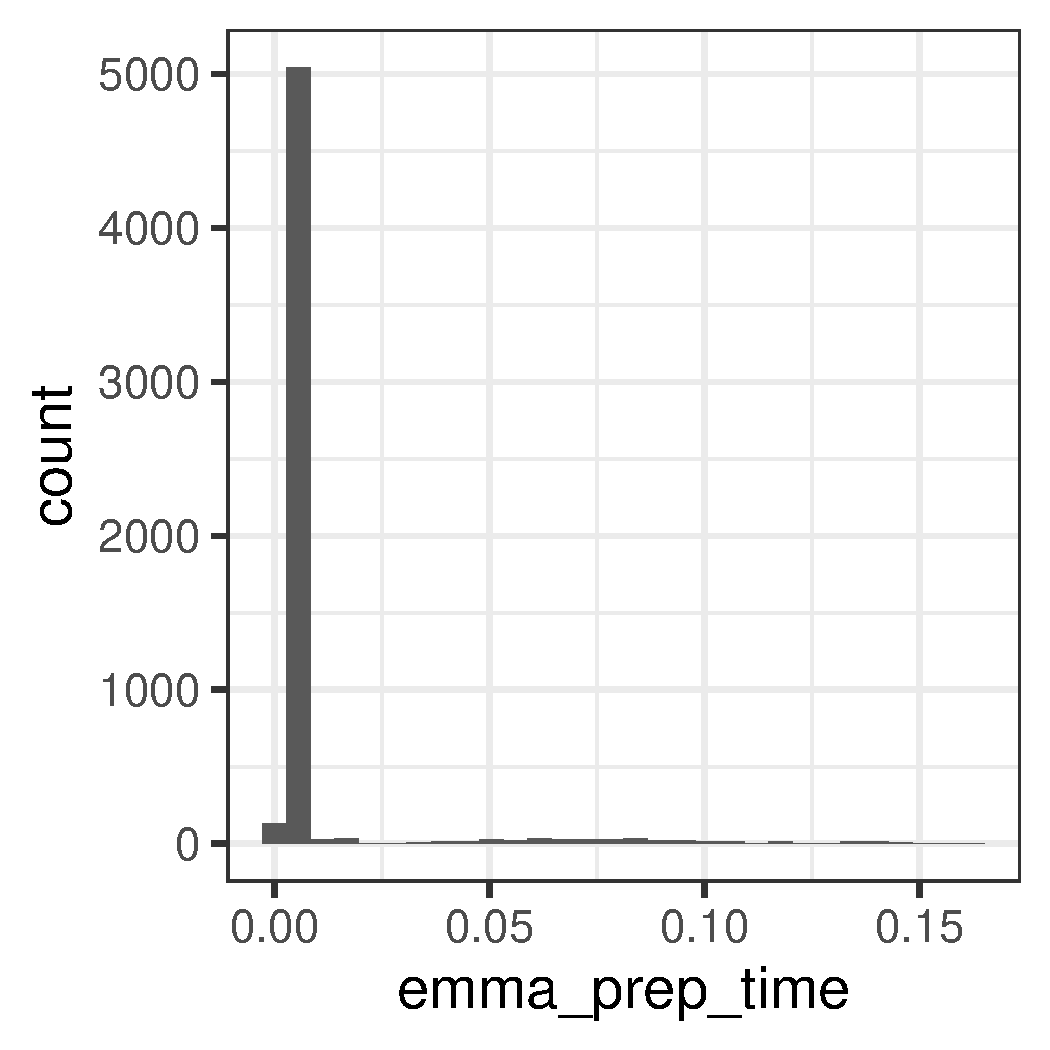
\includegraphics[width=\maxwidth]{figures/figure_staub_exp3unnamed-chunk-22-1} 
\begin{kframe}\begin{alltt}
\hlkwd{ggsave}\hlstd{(}\hlstr{"staub-e.pdf"}\hlstd{,} \hlkwc{width} \hlstd{=} \hlnum{20}\hlstd{,} \hlkwc{height} \hlstd{=} \hlnum{12}\hlstd{)}
\end{alltt}


{\ttfamily\noindent\itshape\color{messagecolor}{\#\# `stat\_bin()` using `bins = 30`. Pick better value with `binwidth`.}}\end{kframe}
\end{knitrout}

\subsection{Prob regression}

\begin{knitrout}
\definecolor{shadecolor}{rgb}{0.969, 0.969, 0.969}\color{fgcolor}\begin{kframe}
\begin{alltt}
\hlcom{############# PARAMS###########}
\hlstd{draws} \hlkwb{<-} \hlkwd{createdraws}\hlstd{(}\hlstr{"prob_regression"}\hlstd{)}

\hlkwd{str}\hlstd{(draws)}
\end{alltt}
\begin{verbatim}
##  num [1:2794, 1:2] 0.122 0.122 0.122 0.122 0.122 ...
\end{verbatim}
\begin{alltt}
\hlkwd{Rhat}\hlstd{(draws)}
\end{alltt}
\begin{verbatim}
## [1] 1.016652
\end{verbatim}
\end{kframe}
\end{knitrout}

Mean etc.

\begin{knitrout}
\definecolor{shadecolor}{rgb}{0.969, 0.969, 0.969}\color{fgcolor}\begin{kframe}
\begin{alltt}
\hlkwd{tail}\hlstd{(draws)}
\end{alltt}
\begin{verbatim}
##              [,1]       [,2]
## [2789,] 0.1451989 0.09932388
## [2790,] 0.1451989 0.09932388
## [2791,] 0.1451989 0.09932388
## [2792,] 0.1451989 0.09932388
## [2793,] 0.1405039 0.11544639
## [2794,] 0.1405039 0.11544639
\end{verbatim}
\begin{alltt}
\hlkwd{mean}\hlstd{(}\hlkwd{c}\hlstd{(draws[,} \hlnum{1}\hlopt{:}\hlnum{2}\hlstd{]))}
\end{alltt}
\begin{verbatim}
## [1] 0.09149012
\end{verbatim}
\begin{alltt}
\hlkwd{median}\hlstd{(}\hlkwd{c}\hlstd{(draws[,} \hlnum{1}\hlopt{:}\hlnum{2}\hlstd{]))}
\end{alltt}
\begin{verbatim}
## [1] 0.0885908
\end{verbatim}
\begin{alltt}
\hlkwd{sd}\hlstd{(}\hlkwd{c}\hlstd{(draws[,} \hlnum{1}\hlopt{:}\hlnum{2}\hlstd{]))}
\end{alltt}
\begin{verbatim}
## [1] 0.03379763
\end{verbatim}
\begin{alltt}
\hlstd{g1} \hlkwb{<-} \hlkwd{ggplot}\hlstd{(}\hlkwd{data.frame}\hlstd{(}\hlkwc{prob_regression} \hlstd{=} \hlkwd{c}\hlstd{(draws[,} \hlnum{1}\hlopt{:}\hlnum{2}\hlstd{])),} \hlkwd{aes}\hlstd{(prob_regression))}
\hlstd{g1} \hlkwb{<-} \hlstd{g1} \hlopt{+} \hlkwd{geom_histogram}\hlstd{()} \hlopt{+} \hlkwd{theme_bw}\hlstd{(}\hlnum{28}\hlstd{)}
\hlstd{g1}
\end{alltt}


{\ttfamily\noindent\itshape\color{messagecolor}{\#\# `stat\_bin()` using `bins = 30`. Pick better value with `binwidth`.}}\end{kframe}
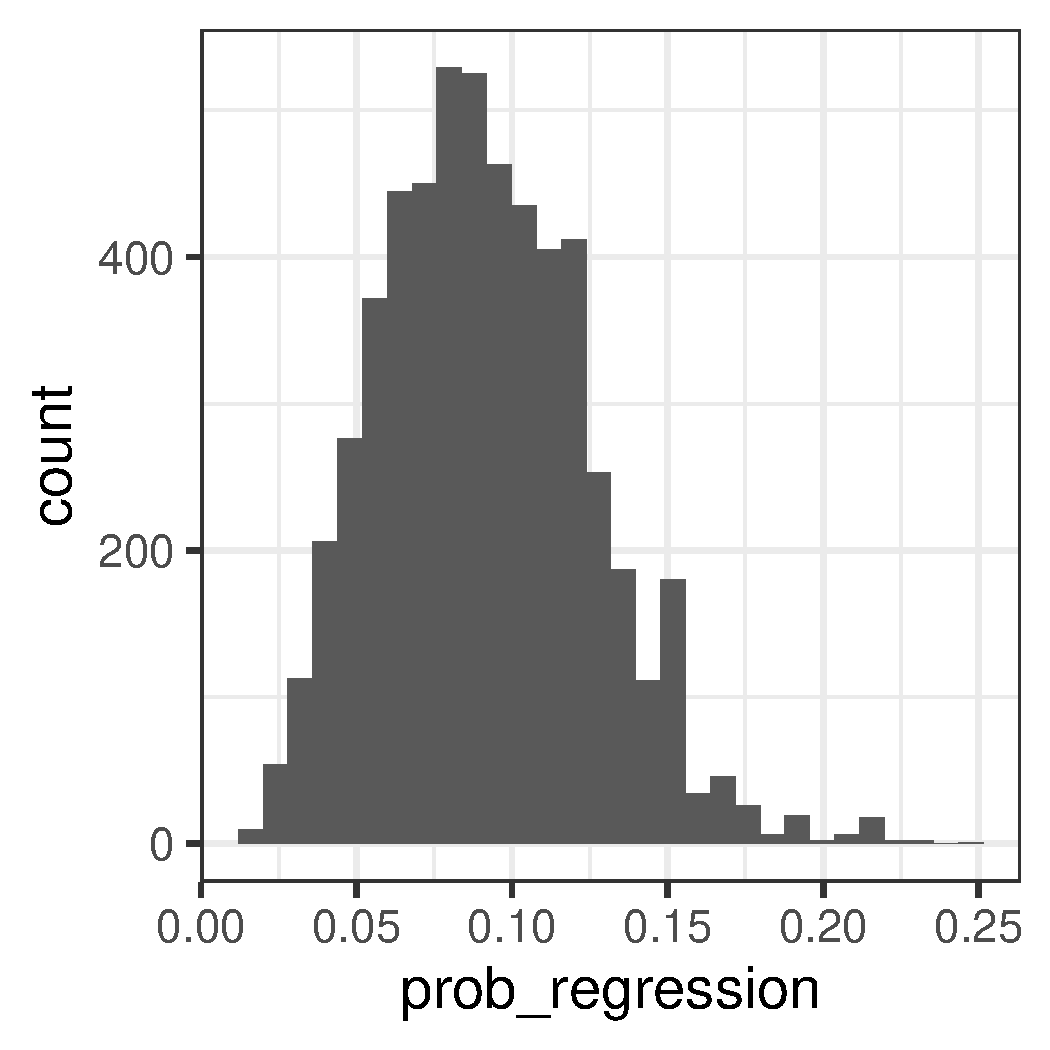
\includegraphics[width=\maxwidth]{figures/figure_staub_exp3unnamed-chunk-24-1} 
\begin{kframe}\begin{alltt}
\hlkwd{ggsave}\hlstd{(}\hlstr{"staub-p.pdf"}\hlstd{,} \hlkwc{width} \hlstd{=} \hlnum{20}\hlstd{,} \hlkwc{height} \hlstd{=} \hlnum{12}\hlstd{)}
\end{alltt}


{\ttfamily\noindent\itshape\color{messagecolor}{\#\# `stat\_bin()` using `bins = 30`. Pick better value with `binwidth`.}}\end{kframe}
\end{knitrout}


\subsection{Threshold}

\begin{knitrout}
\definecolor{shadecolor}{rgb}{0.969, 0.969, 0.969}\color{fgcolor}\begin{kframe}
\begin{alltt}
\hlcom{############# PARAMS###########}
\hlstd{draws} \hlkwb{<-} \hlkwd{createdraws}\hlstd{(}\hlstr{"threshold"}\hlstd{)}

\hlkwd{str}\hlstd{(draws)}
\end{alltt}
\begin{verbatim}
##  num [1:2794, 1:2] 3.45 3.45 3.45 3.48 3.48 ...
\end{verbatim}
\begin{alltt}
\hlkwd{Rhat}\hlstd{(draws)}
\end{alltt}
\begin{verbatim}
## [1] 1.024723
\end{verbatim}
\end{kframe}
\end{knitrout}

Mean etc.

\begin{knitrout}
\definecolor{shadecolor}{rgb}{0.969, 0.969, 0.969}\color{fgcolor}\begin{kframe}
\begin{alltt}
\hlkwd{tail}\hlstd{(draws)}
\end{alltt}
\begin{verbatim}
##             [,1]    [,2]
## [2789,] 3.529291 3.56383
## [2790,] 3.529291 3.56383
## [2791,] 3.529291 3.56383
## [2792,] 3.529291 3.56383
## [2793,] 3.529291 3.56383
## [2794,] 3.529291 3.56383
\end{verbatim}
\begin{alltt}
\hlkwd{mean}\hlstd{(}\hlkwd{c}\hlstd{(draws[,} \hlnum{1}\hlopt{:}\hlnum{2}\hlstd{]))}
\end{alltt}
\begin{verbatim}
## [1] 3.669984
\end{verbatim}
\begin{alltt}
\hlkwd{median}\hlstd{(}\hlkwd{c}\hlstd{(draws[,} \hlnum{1}\hlopt{:}\hlnum{2}\hlstd{]))}
\end{alltt}
\begin{verbatim}
## [1] 3.690112
\end{verbatim}
\begin{alltt}
\hlkwd{sd}\hlstd{(}\hlkwd{c}\hlstd{(draws[,} \hlnum{1}\hlopt{:}\hlnum{2}\hlstd{]))}
\end{alltt}
\begin{verbatim}
## [1] 0.1926334
\end{verbatim}
\begin{alltt}
\hlstd{g1} \hlkwb{<-} \hlkwd{ggplot}\hlstd{(}\hlkwd{data.frame}\hlstd{(}\hlkwc{threshold} \hlstd{=} \hlkwd{c}\hlstd{(draws[,} \hlnum{1}\hlopt{:}\hlnum{2}\hlstd{])),} \hlkwd{aes}\hlstd{(threshold))}
\hlstd{g1} \hlkwb{<-} \hlstd{g1} \hlopt{+} \hlkwd{geom_histogram}\hlstd{()} \hlopt{+} \hlkwd{theme_bw}\hlstd{(}\hlnum{28}\hlstd{)}
\hlstd{g1}
\end{alltt}


{\ttfamily\noindent\itshape\color{messagecolor}{\#\# `stat\_bin()` using `bins = 30`. Pick better value with `binwidth`.}}\end{kframe}
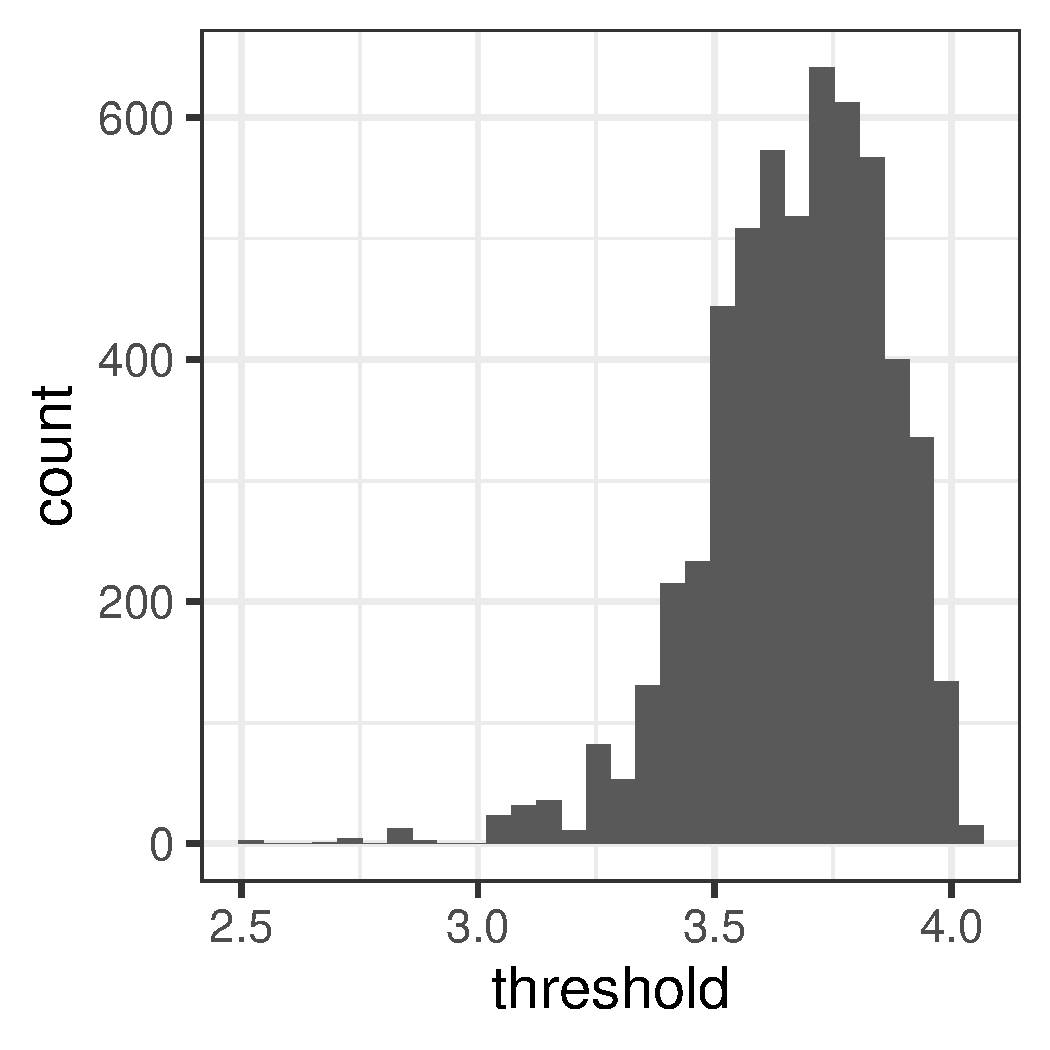
\includegraphics[width=\maxwidth]{figures/figure_staub_exp3unnamed-chunk-26-1} 
\begin{kframe}\begin{alltt}
\hlkwd{ggsave}\hlstd{(}\hlstr{"staub-t.pdf"}\hlstd{,} \hlkwc{width} \hlstd{=} \hlnum{20}\hlstd{,} \hlkwc{height} \hlstd{=} \hlnum{12}\hlstd{)}
\end{alltt}


{\ttfamily\noindent\itshape\color{messagecolor}{\#\# `stat\_bin()` using `bins = 30`. Pick better value with `binwidth`.}}\end{kframe}
\end{knitrout}

\subsection{Std}

\begin{knitrout}
\definecolor{shadecolor}{rgb}{0.969, 0.969, 0.969}\color{fgcolor}\begin{kframe}
\begin{alltt}
\hlcom{############# PARAMS###########}
\hlstd{draws} \hlkwb{<-} \hlkwd{createdraws}\hlstd{(}\hlstr{"std"}\hlstd{)}

\hlkwd{str}\hlstd{(draws)}
\end{alltt}
\begin{verbatim}
##  num [1:2794, 1:2] 45.6 49.4 43.7 28.7 32.6 ...
\end{verbatim}
\begin{alltt}
\hlkwd{Rhat}\hlstd{(draws)}
\end{alltt}
\begin{verbatim}
## [1] 1.000528
\end{verbatim}
\end{kframe}
\end{knitrout}

Mean etc.

\begin{knitrout}
\definecolor{shadecolor}{rgb}{0.969, 0.969, 0.969}\color{fgcolor}\begin{kframe}
\begin{alltt}
\hlkwd{tail}\hlstd{(draws)}
\end{alltt}
\begin{verbatim}
##             [,1]    [,2]
## [2789,] 35.62718 33.0111
## [2790,] 35.62718 33.0111
## [2791,] 35.62718 33.0111
## [2792,] 38.58657 39.7666
## [2793,] 38.58657 39.7666
## [2794,] 35.67267 39.7666
\end{verbatim}
\begin{alltt}
\hlkwd{mean}\hlstd{(}\hlkwd{c}\hlstd{(draws[,} \hlnum{1}\hlopt{:}\hlnum{2}\hlstd{]))}
\end{alltt}
\begin{verbatim}
## [1] 44.73057
\end{verbatim}
\begin{alltt}
\hlkwd{median}\hlstd{(}\hlkwd{c}\hlstd{(draws[,} \hlnum{1}\hlopt{:}\hlnum{2}\hlstd{]))}
\end{alltt}
\begin{verbatim}
## [1] 44.43172
\end{verbatim}
\begin{alltt}
\hlkwd{sd}\hlstd{(}\hlkwd{c}\hlstd{(draws[,} \hlnum{1}\hlopt{:}\hlnum{2}\hlstd{]))}
\end{alltt}
\begin{verbatim}
## [1] 7.442251
\end{verbatim}
\begin{alltt}
\hlstd{g1} \hlkwb{<-} \hlkwd{ggplot}\hlstd{(}\hlkwd{data.frame}\hlstd{(}\hlkwc{std} \hlstd{=} \hlkwd{c}\hlstd{(draws[,} \hlnum{1}\hlopt{:}\hlnum{2}\hlstd{])),} \hlkwd{aes}\hlstd{(std))}
\hlstd{g1} \hlkwb{<-} \hlstd{g1} \hlopt{+} \hlkwd{geom_histogram}\hlstd{()} \hlopt{+} \hlkwd{theme_bw}\hlstd{(}\hlnum{28}\hlstd{)}
\hlstd{g1}
\end{alltt}


{\ttfamily\noindent\itshape\color{messagecolor}{\#\# `stat\_bin()` using `bins = 30`. Pick better value with `binwidth`.}}\end{kframe}
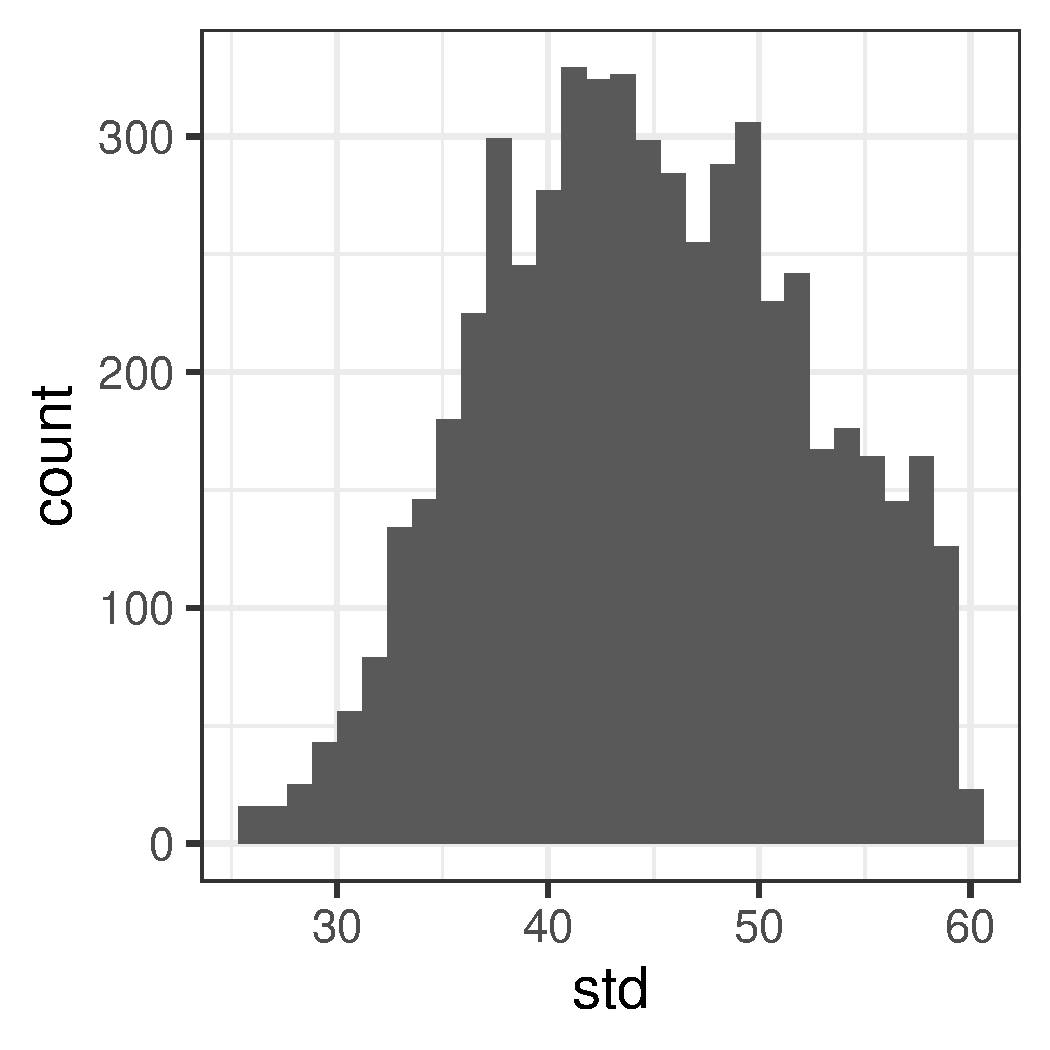
\includegraphics[width=\maxwidth]{figures/figure_staub_exp3unnamed-chunk-28-1} 
\begin{kframe}\begin{alltt}
\hlkwd{ggsave}\hlstd{(}\hlstr{"staub-std.pdf"}\hlstd{,} \hlkwc{width} \hlstd{=} \hlnum{20}\hlstd{,} \hlkwc{height} \hlstd{=} \hlnum{12}\hlstd{)}
\end{alltt}


{\ttfamily\noindent\itshape\color{messagecolor}{\#\# `stat\_bin()` using `bins = 30`. Pick better value with `binwidth`.}}\end{kframe}
\end{knitrout}

\end{document}
